%% BioMed_Central_Tex_Template_v1.06
%%                                      %
%  bmc_article.tex            ver: 1.06 %
%                                       %

%%IMPORTANT: do not delete the first line of this template
%%It must be present to enable the BMC Submission system to
%%recognise this template!!

%%%%%%%%%%%%%%%%%%%%%%%%%%%%%%%%%%%%%%%%%
%%                                     %%
%%  LaTeX template for BioMed Central  %%
%%     journal article submissions     %%
%%                                     %%
%%          <8 June 2012>              %%
%%                                     %%
%%                                     %%
%%%%%%%%%%%%%%%%%%%%%%%%%%%%%%%%%%%%%%%%%


%%%%%%%%%%%%%%%%%%%%%%%%%%%%%%%%%%%%%%%%%%%%%%%%%%%%%%%%%%%%%%%%%%%%%
%%                                                                 %%
%% For instructions on how to fill out this Tex template           %%
%% document please refer to Readme.html and the instructions for   %%
%% authors page on the biomed central website                      %%
%% http://www.biomedcentral.com/info/authors/                      %%
%%                                                                 %%
%% Please do not use \input{...} to include other tex files.       %%
%% Submit your LaTeX manuscript as one .tex document.              %%
%%                                                                 %%
%% All additional figures and files should be attached             %%
%% separately and not embedded in the \TeX\ document itself.       %%
%%                                                                 %%
%% BioMed Central currently use the MikTex distribution of         %%
%% TeX for Windows) of TeX and LaTeX.  This is available from      %%
%% http://www.miktex.org                                           %%
%%                                                                 %%
%%%%%%%%%%%%%%%%%%%%%%%%%%%%%%%%%%%%%%%%%%%%%%%%%%%%%%%%%%%%%%%%%%%%%

%%% additional documentclass options:
%  [doublespacing]
%  [linenumbers]   - put the line numbers on margins

%%% loading packages, author definitions

\documentclass[twocolumn]{bmcart}% uncomment this for twocolumn layout and comment line below
%\documentclass{bmcart}

%%% Load packages
%\usepackage{amsthm,amsmath}
%\RequirePackage{natbib}
%\RequirePackage[authoryear]{natbib}% uncomment this for author-year bibliography
%\RequirePackage{hyperref}
\usepackage[utf8]{inputenc} %unicode support
%\usepackage[applemac]{inputenc} %applemac support if unicode package fails
%\usepackage[latin1]{inputenc} %UNIX support if unicode package fails


\usepackage{booktabs} % For formal tables
\usepackage{graphicx}
\usepackage{xspace}
\usepackage{enumerate}
\usepackage{ragged2e}

\usepackage{lstcustom}




%%%%%%%%%%%%%%%%%%%%%%%%%%%%%%%%%%%%%%%%%%%%%%%%%
%%                                             %%
%%  If you wish to display your graphics for   %%
%%  your own use using includegraphic or       %%
%%  includegraphics, then comment out the      %%
%%  following two lines of code.               %%
%%  NB: These line *must* be included when     %%
%%  submitting to BMC.                         %%
%%  All figure files must be submitted as      %%
%%  separate graphics through the BMC          %%
%%  submission process, not included in the    %%
%%  submitted article.                         %%
%%                                             %%
%%%%%%%%%%%%%%%%%%%%%%%%%%%%%%%%%%%%%%%%%%%%%%%%%
%\def\includegraphic{}
%\def\includegraphics{}



%%% Put your definitions there:
\startlocaldefs
\lstdefinelanguage{Xtext}[]{Java}{
	morekeywords={grammar, with, hidden, generate, as, import, returns, current, terminal, enum},
	keywordstyle=[2]{\textbf},
	morestring=[b]",
	tabsize=2,
	numbers=left, 
	numbersep=2pt,
	numberblanklines=false,
	xleftmargin=2em,
	frame=single,
	framexleftmargin=1.5em
}
\newcommand{\lstXtext}[1]{\lstinline[breaklines=true,language=Xtext,basicstyle=\listingsfontinline,mathescape,literate={\-}{}{0\discretionary{-}{}{}}]\S#1\S}


\lstdefinelanguage{DRL}[]{Java}{
	morekeywords={rule, when, from, accumulate, and, not, in, then, for, int, end},
	keywordstyle=[2]{\textbf},
	morecomment=[l]{//}, 
	morecomment=[s]{/*}{*/}, 
	morestring=[b]",
	tabsize=2,
	numbers=left, 
	numbersep=2pt,
	numberblanklines=true,
	xleftmargin=2em,
	frame=single,
	framexleftmargin=1.5em
}

\lstdefinelanguage{Freemarker}[]{Java}{
	morekeywords={if, assign, else},
	keywordstyle=[2]{\textbf},
	morecomment=[l]{//}, 
	morecomment=[s]{/*}{*/}, 
	morestring=[b]",
	showspaces=false,
	tabsize=2,
	numbers=left, 
	numbersep=2pt,
	numberblanklines=false,
	xleftmargin=2em,
	frame=single,
	framexleftmargin=1.5em
}

\lstdefinelanguage{DSL}[]{Java}{
	morekeywords={rule, type, materials, conditions, cond, values},
	keywordstyle=[2]{\textbf},
	morecomment=[l]{//}, 
	morecomment=[s]{/*}{*/}, 
	morestring=[b]",
	showspaces=false,
	tabsize=2, 
	numbers=left, 
	numbersep=2pt,
	numberblanklines=false,
	xleftmargin=2em,
	frame=single,
	framexleftmargin=1.5em
}

\lstdefinelanguage{Cucumber}[]{Java}{
	morekeywords={Feature, Scenario, Given, And, When, Then},
	keywordstyle=[2]{\textbf},
	morecomment=[l]{//}, 
	morecomment=[s]{/*}{*/}, 
	morestring=[b]",
	showspaces=false,
	tabsize=2,
	numbers=left, 
	numbersep=3pt,
	numberblanklines=false,
	xleftmargin=2em,
	frame=single,
	framexleftmargin=1.5em
}

\lstdefinelanguage{Plugin}[]{Java}{
	morekeywords={plugin, groupId, artifactId, version, executions, execution, id, configuration, seed, qcs, goals, goal},
	keywordstyle=[2]{\textbf},
	morecomment=[l]{//}, 
	morecomment=[s]{/*}{*/}, 
	morestring=[b]",
	showspaces=false,
	tabsize=2
}

\newcommand{\callers}{\emph{high-level rules}\xspace}
\newcommand{\shc}{HLR\xspace}
\newcommand{\hlrdsl}{\textsc{HLRDsl}\xspace}



\endlocaldefs




%%% Begin ...
\begin{document}


%%% Start of article front matter
\begin{frontmatter}

\begin{fmbox}
\dochead{Research}

%%%%%%%%%%%%%%%%%%%%%%%%%%%%%%%%%%%%%%%%%%%%%%
%%                                          %%
%% Enter the title of your article here     %%
%%                                          %%
%%%%%%%%%%%%%%%%%%%%%%%%%%%%%%%%%%%%%%%%%%%%%%

\title{On the Use of Metaprogramming and Domain Specific Languages: An Experience Report in the Logistics Domain}

%%%%%%%%%%%%%%%%%%%%%%%%%%%%%%%%%%%%%%%%%%%%%%
%%                                          %%
%% Enter the authors here                   %%
%%                                          %%
%% Specify information, if available,       %%
%% in the form:                             %%
%%   <key>={<id1>,<id2>}                    %%
%%   <key>=                                 %%
%% Comment or delete the keys which are     %%
%% not used. Repeat \author command as much %%
%% as required.                             %%
%%                                          %%
%%%%%%%%%%%%%%%%%%%%%%%%%%%%%%%%%%%%%%%%%%%%%%

\author[
   addressref={aff1},                   % id's of addresses, e.g. {aff1,aff2}
   corref={aff1},                       % id of corresponding address, if any
   %noteref={n1},                        % id's of article notes, if any
   email={pedro.costa@aluno.unb.br}   % email address
]{\inits{PHT}\fnm{Pedro HT} \snm{Costa}}
\author[
   addressref={aff1},
   corref={aff1},
   email={ednacanedo@unb.br}
]{\inits{ED}\fnm{Edna Dias} \snm{Canedo}}
\author[
	addressref={aff1},
	corref={aff1},
	email={rbonifacio@unb.br}
]{\inits{RB}\fnm{Rodrigo} \snm{Bonif\'{a}cio}}

%%%%%%%%%%%%%%%%%%%%%%%%%%%%%%%%%%%%%%%%%%%%%%
%%                                          %%
%% Enter the authors' addresses here        %%
%%                                          %%
%% Repeat \address commands as much as      %%
%% required.                                %%
%%                                          %%
%%%%%%%%%%%%%%%%%%%%%%%%%%%%%%%%%%%%%%%%%%%%%%

\address[id=aff1]{%                           % unique id
  \orgname{Computer Science Department, University of Bras\'{i}lia - (UnB)}, % university, etc
  \street{P.O. Box 4466},                     %
  \postcode{70910-900}                                % post or zip code
  \city{Bras\'{i}lia},                        % city
  \cny{BR}                                    % country
}


%%%%%%%%%%%%%%%%%%%%%%%%%%%%%%%%%%%%%%%%%%%%%%
%%                                          %%
%% Enter short notes here                   %%
%%                                          %%
%% Short notes will be after addresses      %%
%% on first page.                           %%
%%                                          %%
%%%%%%%%%%%%%%%%%%%%%%%%%%%%%%%%%%%%%%%%%%%%%%

\begin{artnotes}
%\note{Sample of title note}     % note to the article
%\note[id=n1]{Equal contributor} % note, connected to author
\end{artnotes}

%\end{fmbox}% comment this for two column layout

%%%%%%%%%%%%%%%%%%%%%%%%%%%%%%%%%%%%%%%%%%%%%%
%%                                          %%
%% The Abstract begins here                 %%
%%                                          %%
%% Please refer to the Instructions for     %%
%% authors on http://www.biomedcentral.com  %%
%% and include the section headings         %%
%% accordingly for your article type.       %%
%%                                          %%
%%%%%%%%%%%%%%%%%%%%%%%%%%%%%%%%%%%%%%%%%%%%%%

\begin{abstractbox}

\begin{abstract} % abstract
\justify
In this paper we present the main design and architectural decisions to build an enterprise system that deals with the distribution of equipment to the Brazilian Army. The requirements of the system are far from trivial, and we have to conciliate the need to extract business rules from the source code (increasing software flexibility) with the requirements of not exposing the use of declarative languages to use a rule-based engine and simplifying the tests of the application. Considering these goals, we present in this paper a seamless integration of meta-programming and domain-specific languages. The use of meta-programming allowed us to isolate and abstract all definitions necessary to externalize the business rules that ensure the correct distribution of the equipment through the Brazilian Army unities. The use of a domain specific language simplified the process of writing automatic test cases related to our domain. Although our architecture targets the specific needs of the Brazilian Army, we believe that logistic systems from other institutions might also benefit from our technical decisions.
\end{abstract}

%%%%%%%%%%%%%%%%%%%%%%%%%%%%%%%%%%%%%%%%%%%%%%
%%                                          %%
%% The keywords begin here                  %%
%%                                          %%
%% Put each keyword in separate \kwd{}.     %%
%%                                          %%
%%%%%%%%%%%%%%%%%%%%%%%%%%%%%%%%%%%%%%%%%%%%%%

\begin{keyword}
\kwd{Software Architecture}
\kwd{Generative Programming}
\kwd{Domain Specific Languages}
\kwd{Military Logistics}
\end{keyword}

% https://cran.r-project.org/web/classifications/MSC.html
% MSC classifications codes, if any
%\begin{keyword}[class=AMS]
%\kwd[Primary ]{}
%\kwd{}
%\kwd[; secondary ]{}
%\end{keyword}

\end{abstractbox}
%
\end{fmbox}% uncomment this for twcolumn layout

\end{frontmatter}

%%%%%%%%%%%%%%%%%%%%%%%%%%%%%%%%%%%%%%%%%%%%%%
%%                                          %%
%% The Main Body begins here                %%
%%                                          %%
%% Please refer to the instructions for     %%
%% authors on:                              %%
%% http://www.biomedcentral.com/info/authors%%
%% and include the section headings         %%
%% accordingly for your article type.       %%
%%                                          %%
%% See the Results and Discussion section   %%
%% for details on how to create sub-sections%%
%%                                          %%
%% use \cite{...} to cite references        %%
%%  \cite{koon} and                         %%
%%  \cite{oreg,khar,zvai,xjon,schn,pond}    %%
%%  \nocite{smith,marg,hunn,advi,koha,mouse}%%
%%                                          %%
%%%%%%%%%%%%%%%%%%%%%%%%%%%%%%%%%%%%%%%%%%%%%%







%%%%%%%%%%%%%%%%%%%%%%%%% start of article main body
% <put your article body there>

%%%%%%%%%%%%%%%%
%% Background %%
%%



\section{Introduction}\label{sec:Introduction}

Planning and distributing equipment to an army force is a
  challenging task that involves several steps. First, the
  domain experts must specify all material that is relevant
  for a given class (for instance, operational material, official army clothing,
  and army ammunition). Second, domain experts must specify association 
rules that relate military materials to abstract 
organizational unities (e.g., departments, regiments,
and military positions). Third, the domain experts should 
execute the association rules for computing a list of expected
equipment for the \emph{abstract military unit}; and the
designation of the materials that must be
actually distributed to the \emph{concrete military organizations}. Concrete and
abstract military unities often differ because the first may suffer
variations due to the inclusion and suppression of positions
for its particular type of abstract organizational unit.

Decision support systems are essential in this domain, given the importance and complexity of the processes related to the allocation of military employment materials. In particular, the rules used to predict military materials and equipment are not trivial, and implementing these rules directly in the source code makes the systems difficult to understand and maintain. This problem mostly occurs because the number of conditions that need to be expressed is proportional to the complexity of the organizational structure and the number of materials. In the case of an entire army force (such as the Brazilian Army), this number is noteworthy. In addition, a ``\emph{hard-coding}'' solution does not allow domain experts to trivially specify and test new derivation rules. For these reasons, it is preferably to implement these rules declaratively, using languages, tools, or libraries that
support inference mechanisms.

However, it is anything but easy to introduce either a logic language (e.g., Prolog or Datalog) or a specific library (such as Drools~\cite{browne2009}) in a complex enterprise system---particularly in environments whose whole ecosystem is well established and based on a set of constraints related to both language and libraries usage. Furthermore, these solutions require a steep learning curve, and thus it is worth to modularize and abstract their usage in the architecture of enterprise systems.

In a previous work we describe the main design and architectural decisions we had taken to implement the mechanisms that assist decision makers to plan the distribution of military materials and equipment across the organizational structure of the Brazilian Army~\cite{phtcosta:sbcars}. These decisions aim to both (a) abstract the adoption of a business rule engine using {\bf meta-programming} and (b) allow domain experts to simulate the definition and testing of rules using a {\bf domain specific language} (DSL). Altogether, previously we contributed with:

\begin{enumerate}[(a)] 

\item A description of the use of generative programming techniques to raise the abstraction level related to the adoption of a logic programming language in the specification of rules for the 	distribution of materials and equipment through organizational unities.

\item A report of an empirical evaluation of our design and architectural decisions, reinforcing that they fulfill not only the needs of the domain specialists, but also existing technical constraints. 	

\end{enumerate}


In this paper we extend our previous work with a more detailed description of our DSL \textcolor{red}{and an in depth evaluation of our approach}---considering the results of a property based testing execution. We complemented this evaluation through a qualitative assessment using the focus group method. The goal of this comprehensive assessment was to collect more evidence about how our approach fulfills the functional requirement of correctly distributing equipment to military units, by considering a more systematic testing technique and the opinion of domain experts responsible for planing the distribution of operational material in the Brazilian Army. 

Although we discuss the distribution of materials and equipment for the military domain (which is far from trivial), we believe that the architectural decisions discussed here can be exploited to other logistics and endorsements scenarios in which it is also desirable to transparently introduce the support for rule based engines in enterprise systems.

\textcolor{red}{This paper is organized as follows. The Section \ref{sec:logistics} presents the concepts related to the domain of material logistics. Section \ref{sigelog} presents the concepts related to business rules and rule based engines and Section \ref{back} presents some background information related to generative programming—techniques that we use to support the design and implementation of our approach. Section \ref{sec:Methodology} explains the research methodology used. Section \ref{sec:architecture} presents the main design and architectural decisions we take to develop the mechanism responsible for the distribution of materials. In Section \ref{sec:case_study} we present the results of an empirical study that validate our approach. Section \ref{threats} presents the discussion and threats to validity this work. Finally, Section \ref{sec:related} and Section \ref{sec:conclusao} relate our work with the existing literature and present some final remarks.}



%%%%%%%%%%%%%%%%%%%%%%%%%%%%%%
%% Military Logistics Systems
%%%%%%%%%%%%%%%%%%%%%%%%%%%%%%
\section{Military Logistic Domain}
\label{sec:logistics}

Military Logistics is the method used to implement military strategies and tactics that aim to gain competitive advantage~\cite{rutner2012}. Logistics is defined as the art of moving armies, as well as accommodating and supplying the military~\cite{prebilic2006}. Strategy and tactics provide the framework for conducting military operations, while logistics provides the means. In the context of this paper, we are more interested in the supplying aspects of logistics, which refers to the set of activities that deals with the  provisioning of the material of different classes (including vehicles, armaments, munition, uniform, and fuel) necessary to the military unities (including a rich organizational structure and a significant number of militaries). 

In order to facilitate the administration and control of materials and equipment, the Brazilian Army uses a catalog system that is similar to one defined by the North Atlantic Treaty Organization (NATO)~\cite{otan2012}, which classifies items into groups and classes. The Brazilian Army catalog uses a classification that considers the \emph{type}, \emph{class}, and \emph{family} of the materials, ignoring some details (such as specific brands and suppliers). Other areas of the logistic domain consider more detailed information of the equipment. Several rules govern the identification of materials and equipment, to avoid duplication and simplify the process of decision making. A logistic system is the integrated set of organizations, personnel, principles, and technical standards intended to provide the adequate flow for supplying materials~\cite{brasil2003}. This is a complex system, and thus it must be designed as a set of modules. 

In this paper we present the main design and architectural decisions related to one of the modules (SISDOT) of the \emph{Integrated Logistics System} (SIGELOG) of the Brazilian Army. SISDOT deals with the identification of the necessary materials and equipment (hereafter MEMs) for the organizational unities of the Brazilian Army. Each organizational unity is a combination of a set of \emph{generic organizations of specific types}, which describe the expected number of military unities of an organization (including armies, divisions, brigades, and so on). The goal of SISDOT is twofold. It first estimates the set of MEMs that should be assigned to the generic organizations, producing one of its main products (named QDM). Based on a set of QDMs, the second SISDOT's goal is to derive another estimate of MEMs that should be assigned to the concrete organizational unities (a QDMP). 

Before generating a QDM, it is necessary to catalog all relevant MEMs to a given class of materials and then specify \callers (HLRs) that relate MEMs to the generic organizational unities, considering different elements of the structure---from the type of the unity and sub-unities to the qualifications of a soldier. That is, it is possible to elaborate a \shc that states that a military ambulance should be assigned to all \emph{drivers within medical unities}. Differently, it is also possible to state that an automatic rifle will be assigned to all \emph{sergeant that has been qualified as a shooter}. There is some degree of flexibility for writing these rules, that might be from two different kinds: rules that consider the entire structure of the Brazilian Army and rules that refer to specific elements of the organizational structure. The former details rules that are more specific for a set of military qualifications. The second allows the generation of rules that might be reused through different unities. 

Deriving QDMs and QDMPs is not trivial and its complexity is due to several factors, including the organizational structure of the Brazilian Army, the number of existing functions and qualifications that must be considered, and the reasonable number of MEMs. The process might also vary depending on the class of the materials. Moreover, it is possible to specify the \callers in different ways, which might interact to each other leading to undesired results (e.g., the same material being assigned several times to a given soldier). 

\section{SIGELOG Architectural Constraints}
\label{sigelog}

Due to the number of logical decisions, using an imperative language to implement the process of QDM generation 
is not an interesting choice. However, the SIGELOG architecture reinforces the use of Java Enterprise Edition platform---so we had little flexibility to introduce a more suitable language (such as Prolog) to generate QDMs. Other constraints guided the architectural decisions of SISDOT, including:  

\begin{itemize}
	\item Maintenance: the set of languages and libraries are limited to those already used in the SIGELOG development.  
	\item Performance: considering a total of 1000 \callers, the system must be able to generate a QDM in less than 10 seconds.
	\item Testing: the technical decisions must not compromise the testability of the system, being expected a high degree of automated tests. 
\end{itemize}

To deal with the first constraint, we decided to use a meta-programming approach that derives \emph{low-level rules} for Drools (a rule based engine for Java) \emph{on the fly}, from a set of \callers represented as domain objects that must exist in a database. In this way, it is not necessary to understand the language used to specify rules in Drools.

To this end, we generate all low-level rules every time a QDM is built.
Although this approach increases flexibility and allows us to externalize the \emph{low-level rules}, we realized some undesired effect on the performance of the system. Accordingly, to deal with the second constraint, we use a cache mechanism and, based on the results of performance tests (as we discuss in Section~\ref{sec:case_study}), we have evidences that we are able to generate QDMs within the time
limit constraints. For the third constraint, we implemented a DSL that simplifies the specification and execution of test cases using a property based approach. 


\section{Technical Background}
\label{back}


In this section we
introduce some technical background related to \emph{Rule Based Systems} and
\emph{Drools}, \emph{Generative Programming} (including \emph{Metaprogramming},
\emph{Template Engines}, and \emph{Domain Specific Languages}), and
\emph{Property Based Testing}. This background might help the reader to
understand the design and architectural decisions we take
while implementing SISDOT.  
%%%%%%%%%%%%%%%%%%%%%%%%%%%%%%
%% Rule Based Systems
%%%%%%%%%%%%%%%%%%%%%%%%%%%%%%
\subsection{Rule Based Systems}
\label{sec:rbs}
The process for deriving QDMs consists of applying a set of business rules that relates MEMs to the organizational structure of the Brazilian Army. In this paper, we named this set of business rules as \callers. A business rule is a compact, atomic, and well-formed statement about an aspect of the business that can be expressed in terms that may be directly related to the business and its employees using a simple and unambiguous language that might be accessible to all stakeholders~\cite{graham2007business}. This type of structure is relevant for the organizations, as they continuously need to deal with complex scenarios. These scenarios consist of a large number of individual decisions, working together to provide a complex assessment of the organization as a whole \cite{salatino2016mastering}.

Rule Based Systems (RBS), also known as production systems or expert systems, are the simplest form of artificial intelligence that help to design solutions that reason about and take actions from business rules (a feature that is interesting in the context of SISDOT), using rules such as knowledge representation~\cite{grosan2011}. Instead of representing knowledge in a declarative and static way as a set of things that are \emph{true}, RBS represent knowledge in terms of a set of rules that tells what to do or what to accomplish in different situations~\cite{grosan2011}. RBS consist of two basic elements: a \emph{knowledge base} to store knowledge and an \emph{inference engine} that implements  algorithms to manipulate the knowledge represented in the knowledge base~\cite{grosan2011,DBLP:books/daglib/0070547,gallacher1989}. The knowledge base stores facts and rules~\cite{DBLP:journals/cacm/Hayes-Roth85}. A fact is a static statement about properties, relations, or propositions~\cite{DBLP:journals/cacm/Hayes-Roth85} and should be something relevant to the initial state of the system~\cite{grosan2011}. A rule is a conditional statement that links certain conditions to actions or results \cite{abraham2005}, being able to express policies, preferences, and constraints. Rules can be used to express deductive knowledge, such as logical relationships, and thus support inference, verification, or evaluation tasks~\cite{DBLP:journals/cacm/Hayes-Roth85}.

A rule ``if-then'' takes a form like \emph{``if x is A then take a set of actions''}. The conditional part is known as antecedent, premise, condition, or left-hand-side (LHS). The other part is known as consequent, conclusion, action, or right-hand-side (RHS)~\cite{grosan2011,abraham2005}. Rule-based systems works as follows~\cite{grosan2011}: it starts with a knowledge base, which contains all appropriate knowledge coded using ``if-then'' rules, and a working memory, which contains all data, assertions, and information initially known. 

The system examines all rule conditions (LHS) and determines a subset of rules whose conditions are satisfied, based on the data available at the working memory. From this information set, some of the rules are triggered. The choice of rules is based on a conflict resolution strategy. When the rule is triggered, all actions specified in its \texttt{then} clause (RHS) are executed. These actions can modify the working memory, the rule base itself, or take whatever action that the system programmer decides to implement. This \emph{trigger rule loop} continues until a termination criterion is met. This end criterion can be given by the fact that there is not any additional rule whose conditions are satisfied or a rule is triggered whose action specifies that the program should be finished.

Drools is an example of a business logic integration platform (BLiP) written in the Java programming language and that fits some requirements of SISDOT (in particular, its integration with Java and the Wildfly application server). We use Drools as the \emph{rule-based system} in the QDM generation. However, to abstract the use of a RBS, we generate the Drools rules using a meta-programming approach, a specific technique for \emph{generative programming}. 




%%%%%%%%%%%%%%%%%%%%%%%%%%%%%%
%% Generative Programming
%%%%%%%%%%%%%%%%%%%%%%%%%%%%%%
\subsection{Generative Programming}
\label{sec:gp}

Generative Programming (GP) is related to the design and implementation of software components that can be combined to generate specialized and highly optimized systems, fulfilling specific requirements~\cite{DBLP:phd/dnb/Czarnecki99}. With this approach, instead of developing solutions from scratch, domain-specific solutions are generated from reusable software components \cite{arora2009}. GP is applied on the manufacturing of software products from components in a system in an automated way (and within economic constraints), i.e., using an approach that is similar to that found in industries that have been producing mechanical, electronic, and other goods for decades \cite{barth2002}. The main idea in GP is similar to the one that led people to switch from Assembly languages to high-level languages. 

In our context, we use GP to deal with two different aspects of SISDOT. First, we raise the level of abstraction by automatically generating low-level Drools rules from an existing set of \callers (previously defined by the domain experts). This is a \emph{meta-programming} approach based on template engines---we use a template to generate a set of facts and rules (which are the fundamental mechanisms of logic programming) from domain objects. We also raise the level of abstraction to assist developers in the specification and execution of test cases, using a domain specific language and a set of custom libraries and tools.  


\subsubsection{Metaprogramming and Template Engines}

Metaprogramming concerns to the implementation of programs that generate other programs. In the context of SISDOT, we use a metaprogramming technique to generate programs that are interpreted by Drools. The main goal is to abstract the use of a specific language for implementing the \emph{low-level rules} used to generate QDMs. There are many different approaches for metaprogramming, including preprocessing, source to source transformations, and template engines. A template engine is a generic tool for generating textual output from templates and data files. They can be used in the development of software that requires the automatic generation of code according to specific purposes~\cite{benato2017}. 

The need for dynamically generated web pages has led to the development of numerous template engines in an effort to make web application development easier, improve flexibility, reduce maintenance costs, and enable parallel encoding and development using HTML like languages. In addition to being widely used in dynamic web page generation, templates are used in other tasks, being one of the main techniques to generate source code from high level specifications. More recently, languages such as Clojure, Ruby, Scala, and Haskell adopted the use of template and \emph{quasiquote} mechanisms as a strategy for code reuse and program generation (some of them considering type systems). A template is a text document that combines placeholders and linguistic formulas used to describe something in a specific domain~\cite{segura2017}. 

In this work we use the FreeMarker template engine, which is an open-source software designed to generate text from templates~\cite{radjenovic2009}. FreeMarker was chosen for several reasons, such as: it follows a general purpose model; it is faster than other template engines; it supports shared variables and model loaders; and it is possible to load FreeMarker templates at runtime, without the need to (re)compile the application~\cite{benato2017,parr2006}.


\subsubsection{Domain Specific Languages}

A language is a set of valid sentences, serving as a mechanism for expressing intentions \cite{parr2010}. Creating a new language is a time-consuming task, requires experience, and is usually performed by engineers specialized in languages construction~\cite{karsai2014}. To implement a language, one must construct an application that reads sentences and reacts appropriately to the phrases and input symbols it discovers. However, the need for new languages for many growing domains is increasing, as well as the emergence of more sophisticated tools that allow software engineers to define a new language with acceptable effort. As a result, a growing number of DSLs are being developed to increase developer productivity within specific domains~\cite{karsai2014}. 


Domain Specific Languages (DSL) are specification languages or programming languages with high level of abstraction, simple and concise \cite{raja2010}, focused on specific domains, and are designed to facilitate the construction of applications, usually declaratively, with limited expressiveness lines of code, which solve these specific problems \cite{neeraj2017}. A DSL is a computer language of limited expressiveness, through appropriate notations and abstractions, focused and generally restricted to a specific problem domain \cite{fowler2013,vanDeursen2000}. DSLs have the potential to reduce the complexity of software development by increasing the level of abstraction for a domain. According to the application domain, different notations (textual, graphical, tabular) are used \cite{pfeiffer2008}.


In this work we used Xtext ~\cite{eysholdt2010} (a language workbench) to implement a DSL that helps developers to specify and execute test cases related to the process of QDM generation. The main rationale to building this DSL was the significant costs related to specifying \callers (particularly during acceptance testing).
Our DSL integrates with a \emph{property based testing} infrastructure that
is able to generate different configurations of \emph{military unities}. We use
this infrastructure to increase our confidence about the generation process of
QDMs and support regression testing.


%%%%%%%%%%%%%%%%%%%%%%%%%%%%%%
%% Software Testing
%%%%%%%%%%%%%%%%%%%%%%%%%%%%%%
\subsection{Property Based Software Testing}
\label{sec:test}

% Conforme discutido anteriormente, o uso de uma infraestrutura baseda em Property-based Testing (PBT) consiste em outra decisão arquitetural relevante para o SISDOT. PBT tornou-se uma técnica padrão para melhorar a qualidade do \textit{software} em uma ampla variedade de linguagens de programação \cite{lampropoulos2017}. PBT é uma técnica de teste de caixa-preta, semi-automática, de alto nível na qual, ao invés de escrever um conjunto rico testes de unidade manualmente, o testador especifica propriedades gerais que o sistema sob teste (System Under Testing - SUT) deve satisfazer. A partir dessas propriedades, geradores de dados produzem entradas aleatórias bem distribuídas para as partes do sistema que serão testadas. As propriedades são então verificadas a partir de um conjunto mais rico de entradas, que dificilmente seria explorado manualmente. Como em todas as técnicas de testes aleatórios, a chance de encontrar um erro e a confiança no SUT aumentam com o número de testes gerados \cite{loscher2018}. 

As discussed earlier, another relevant architectural decision of
SISDOT is the use of a Property Based Testing (PBT) infrastructure.
PBT is a model-based testing approach that is getting a lot of attention.
Its main focus is on automatically generating test cases from specifications in the form of high-level
properties~\cite{claessen2000,earle2014,castro2015}. That is, PBT tools and libraries (such as Haskell QuickCheck,
JUnit QuickCheck, C Theft and Scala Test) allow developers and testers to write
program specifications in the form of properties that must be satisfied. From these specifications,
these tools automatically generate input data, execute the test cases, and verify the results of a
large number of random scenarios~\cite{castro2015}.


%% PBT has become a standard technique for improving the quality of software in a wide variety of programming languages \cite{lampropoulos2017}. PBT is a high-level, semi-automatic, black-box testing technique in which, rather than writing a rich set of unit tests manually, the tester specifies general properties that the System Under Testing (SUT) must meet. From these properties, data generators produce well-distributed random inputs for the parts of the system that will be tested. The properties are then checked from a richer set of entries, which would hardly be exploited manually. As with all random testing techniques, the chance of finding an error and confidence in SUT increases with the number of tests generated \cite{loscher2018}.

% PBT é uma técnica que está recebendo muita atenção recentemente, é fortemente relacionada a testes baseados em modelos, mas onde o foco está na geração de testes individuais automaticamente a partir de especificações na forma de testes de propriedades de alto nível \cite{earle2014}. PBT é uma estratégia que leva a uma família de ferramentas de teste automáticas. Geralmente, são ferramentas para geração e execução de casos de teste com base nas especificações. Essas ferramentas são tipicamente implementadas como bibliotecas, permitindo que o desenvolvedor / testador anote as especificações do programa, usando uma linguagem de programação de sua escolha, na forma de propriedades que devem ser satisfeitas. A partir dessas especificações, as ferramentas geram, executam e verificam automaticamente os resultados de um grande número de casos de teste aleatórios para verificar se as propriedades são mantidas \cite{castro2015}. Existe uma variedade de ferramentas PBT que surgiram ao longo dos anos inspiradas no QuickCheck original para Haskell \cite{claessen2000}, como: JUnit-QuickCheck para Java, theft para C, ScalaTest and ScalaCheck para Scala \cite{chepurnoy2018}. 


% Ao contrário dos métodos de teste convencionais, em que o comportamento de um programa é testado apenas em alguns casos pré-determinados, o PBT enfatiza a definição de propriedades e, em seguida, testa sua validade em relação a pontos de dados amostrados aleatoriamente. Como o teste baseado em propriedade (PBT) usa um pequeno número de pontos de dados amostrados aleatoriamente, ele ainda fornece apenas uma resposta aproximada à questão de saber se uma propriedade é satisfeita em todos os pontos de dados. No entanto, pode fornecer mais confiança do que o teste unitário convencional, porque os pontos de dados amostrados aleatoriamente podem cobrir casos problemáticos que não foram previstos pelos desenvolvedores \cite{chepurnoy2018}.

%% Unlike conventional test methods, where the behavior of a program is tested only in a small number of cases,
%% the PBT approach emphasizes the definition of properties and then tests its validity against randomly sampled data points. Because the property-based test (PBT) uses a small number of randomly sampled data points, it still provides only a rough answer to the question of whether a property is satisfied at all data points. However, it can provide more confidence than the conventional unit test, because randomly sampled data points can cover problematic cases that were not anticipated by developers \cite{chepurnoy2018}.

% PBT apresenta três vantagens sobre o teste manual \cite{yatoh2014}. Primeiro, escrevendo apenas propriedades e omitindo dados de teste, os desenvolvedores podem reduzir significativamente o tamanho e complexidade do código de teste. Segundo, ao executar testes baseados em propriedade contra entradas geradas aleatoriamente, os desenvolvedores podem encontrar mais \textit{bugs} do que testes manuais, pois os testes baseados em propriedade podem verificar propriedades com muitas entradas, com isso, a chance de encontrar \textit{bugs} é aumentada. Finalmente, as propriedades podem ser vistas como uma especificação formal leve do programa. Escrever especificações formais promove o entendimento da especificação e da implementação e é eficaz para compartilhar as especificações entre a equipe. É importante que essa especificação seja executável. Essa especificação executável pode evitar incompatibilidade entre especificação e implementação, o que geralmente é o caso se a especificação for gravada em um documento separado.

PBT has three advantages over conventional testing approaches~\cite{yatoh2014}. First, by writing only properties and omitting test data, developers can significantly reduce the size and complexity of the test code. Second, when running property-based tests against randomly generated input data, the likelihood to find bugs might increase. Lastly, the approach can be understood as a lightweight formal specification of the program, which might help to further understand the system. Here we particularly benefited from the first and second expected outcomes of using PBT.  

  
% O estudo realizado por \cite{elberzhager2012} identifica abordagens existentes para reduzir o esforço de teste sem que o software final perca qualidade. A maioria dos artigos analisados, cerca de 50\%, discute a automação de testes. Na literatura são descritas diversas técnicas para geração de casos de testes e dados para testes, como as apresentadas em \cite{hooda2014}, \cite{mahadik2016}, \cite{elghondakly2016}, \cite{ali2010}, \cite{harman2010}, \cite{sahoo2016}, \cite{khurana2017}.

%% The study by \cite{elberzhager2012} identifies existing approaches to reduce the test effort without the final software losing quality. Most articles reviewed, about 50\%, discuss automation testing. In the literature, several techniques are described for the generation of test cases and data for tests, such as those presented \cite{hooda2014}, \cite{mahadik2016}, \cite{elghondakly2016}, \cite{ali2010}, \cite{harman2010}, \cite{sahoo2016}, \cite{khurana2017}.

%% {\color{red}talvez esse primeiro paragrafo possa ser o primeiro paragrafo da secao 4.3}

% Para este estudo foi selecionada a técnica PBT devido às características dos chamadores, que diferem entre si basicamente pelas suas propriedades declaradas e seus valores. Uma ferramenta bastante conhecida, o Junit QuickCheck \footnote{https://pholser.github.io/junit-quickcheck/site/0.8.2/index.html}, foi levada em consideração para uso. Embora exista uma documentação para esta ferramenta não foi possível encontrar exemplos que tornassem sua utilização mais clara no caso do SISDOT. Além disso, pode ser difícil entender os artefatos gerados em tempo de execução{\color{red}, pois não seria possível saber exatamente quais valores de propriedades estão sendo testados, a não ser pela leitura do log de execução.} Foram encontradas outras ferramentas, como: jqwik \footnote{https://jqwik.net/} e QuickTheories \footnote{https://github.com/ncredinburgh/QuickTheories}, mas que também incorrem nos mesmos problemas, mesmo que não tenham sido analisadas mais a fundo como o Junit QuickCheck.

In particular, we decided to use a PBT technique due to the characteristics of the \callers,
which differ by their properties and values. A manual approach for generating different combinations
of properties and value is time consuming. We first considered the use of Junit QuickCheck.\footnote{https://github.com/pholser/junit-quickcheck} However, due to limited documentation, we could not find examples that would make clear its use in the case of SISDOT.
Furthermore, we need control on the procedures for generating data,
and we found that implementing
our own infrastructure would be more feasible than trying to adapt the Junit QuichCheck to this end. Other tools were considered as well
(such as: jqwik \footnote{https://jqwik.net/} and QuickTheories \footnote{https://github.com/ncredinburgh/QuickTheories}),
but we found that they would also incur in the same problems.

% O PBT é uma abordagem poderosa para testes de software, mas pode ser tão desafiadora para desenvolvedores que a usam pela primeira vez quanto para os stakeholders não técnicos entenderem, em geral, os artefatos gerados. Abordagens ágeis para o desenvolvimento de software, como a utilizada no desenvolvimento do SISDOT, demonstram que o envolvimento de todas as partes interessadas no ciclo de vida do software é um fator-chave para o sucesso do projeto. Especificamente, permitir que clientes ou usuários validem os requisitos de software por inspeção direta ou mesmo interação com artefatos de garantia de qualidade de software, como casos de testes e conjunto de testes, traz benefícios efetivos \cite{castro2016}. Neste trabalho, para facilitar o envolvimento dos stakeholders, foi desenvolvida uma solução própria, em detrimento às ferramentas existentes, baseada em PBT, que gera, além de outros artefatos, especificações de teste baseadas no Cucumber \cite{wynne2017}, possibilitando o entendimento de todos os envolvidos sobre o que está sendo testado.

%% PBT is a powerful approach to software testing, but it can be so challenging for developers who use it for the first time as non-technical stakeholders generally understand the artifacts they generate. Agile approaches to software development, such as that used in the development of SISDOT, demonstrate that engaging all stakeholders in the software life cycle is a key factor for project success. Specifically, allowing customers or users to validate software requirements by direct inspection or even interaction with software quality assurance artifacts, such as test cases and test suite, brings effective benefits \cite{castro2016}. In order to facilitate stakeholder engagement, a proprietary solution was developed over PBT-based tools that generate, in addition to other artifacts, test specifications based on Cucumber \cite{wynne2017}, allowing the understanding of all involved about what is being tested.

%% {\color{red}In the next section we present more details about our architectural decisions and implementation of our metaprogramming and DSL approach, which deals with the generation and test of QDMs.}




%%%%%%%%%%%%%%%%%%%%%%%%%%%%%%%%%%%%%%%%%%%%%%
%% Architectural Decisions
%%%%%%%%%%%%%%%%%%%%%%%%%%%%%%%%%%%%%%%%%%%%%%
\section{Architectural Decisions}
\label{sec:architecture} 

SISDOT is based on the client-server architectural style (according to a typical Java enterprise application), where the components interact to each other by requesting services from other components~\cite{clements2011documenting}. SISDOT is also organized into logical groups of components (known as tiers)---a strategy often used in the client-server architectural style. The multi-tier architectural pattern can be classified as a \emph{component and connector} pattern, depending on the criterion used to define the tiers~\cite{bass2013software}. Indeed, there are several criteria, such as component type, sharing of the execution environment, 
and so on~\cite{clements2011documenting}.

The multi-tier pattern also induces some topological constraints that govern how the components might interact with other components. 
Specifically, connectors might only exist between components of the same tier or that reside in an adjacent tier~\cite{clements2011documenting}. In addition, according to Bass et al., the organization of a system using tiers supports software maintenance, facilitates the definition of security policies, and might increase the performance, availability, and modifiability of 
the systems~\cite{bass2013software}. 



%%%%%%%%%%%%%%%%%%%%%%%%%%%%%%
%% Runtime Architectural Description for QDM Generation
%%%%%%%%%%%%%%%%%%%%%%%%%%%%%%
\subsection{Runtime Architectural Description for QDM Generation}

In order to further detail and illustrate the SISDOT architecture, and the main architectural decisions to address the constraints introduced in Section~\ref{sec:logistics}, here we present a scenario that refers to the generation of QDMs using a runtime architectural description, whose components, relationships, and interactions are illustrated in Figure~\ref{fig:runtime_qdm}). 

\begin{figure}[!ht] %\centering
	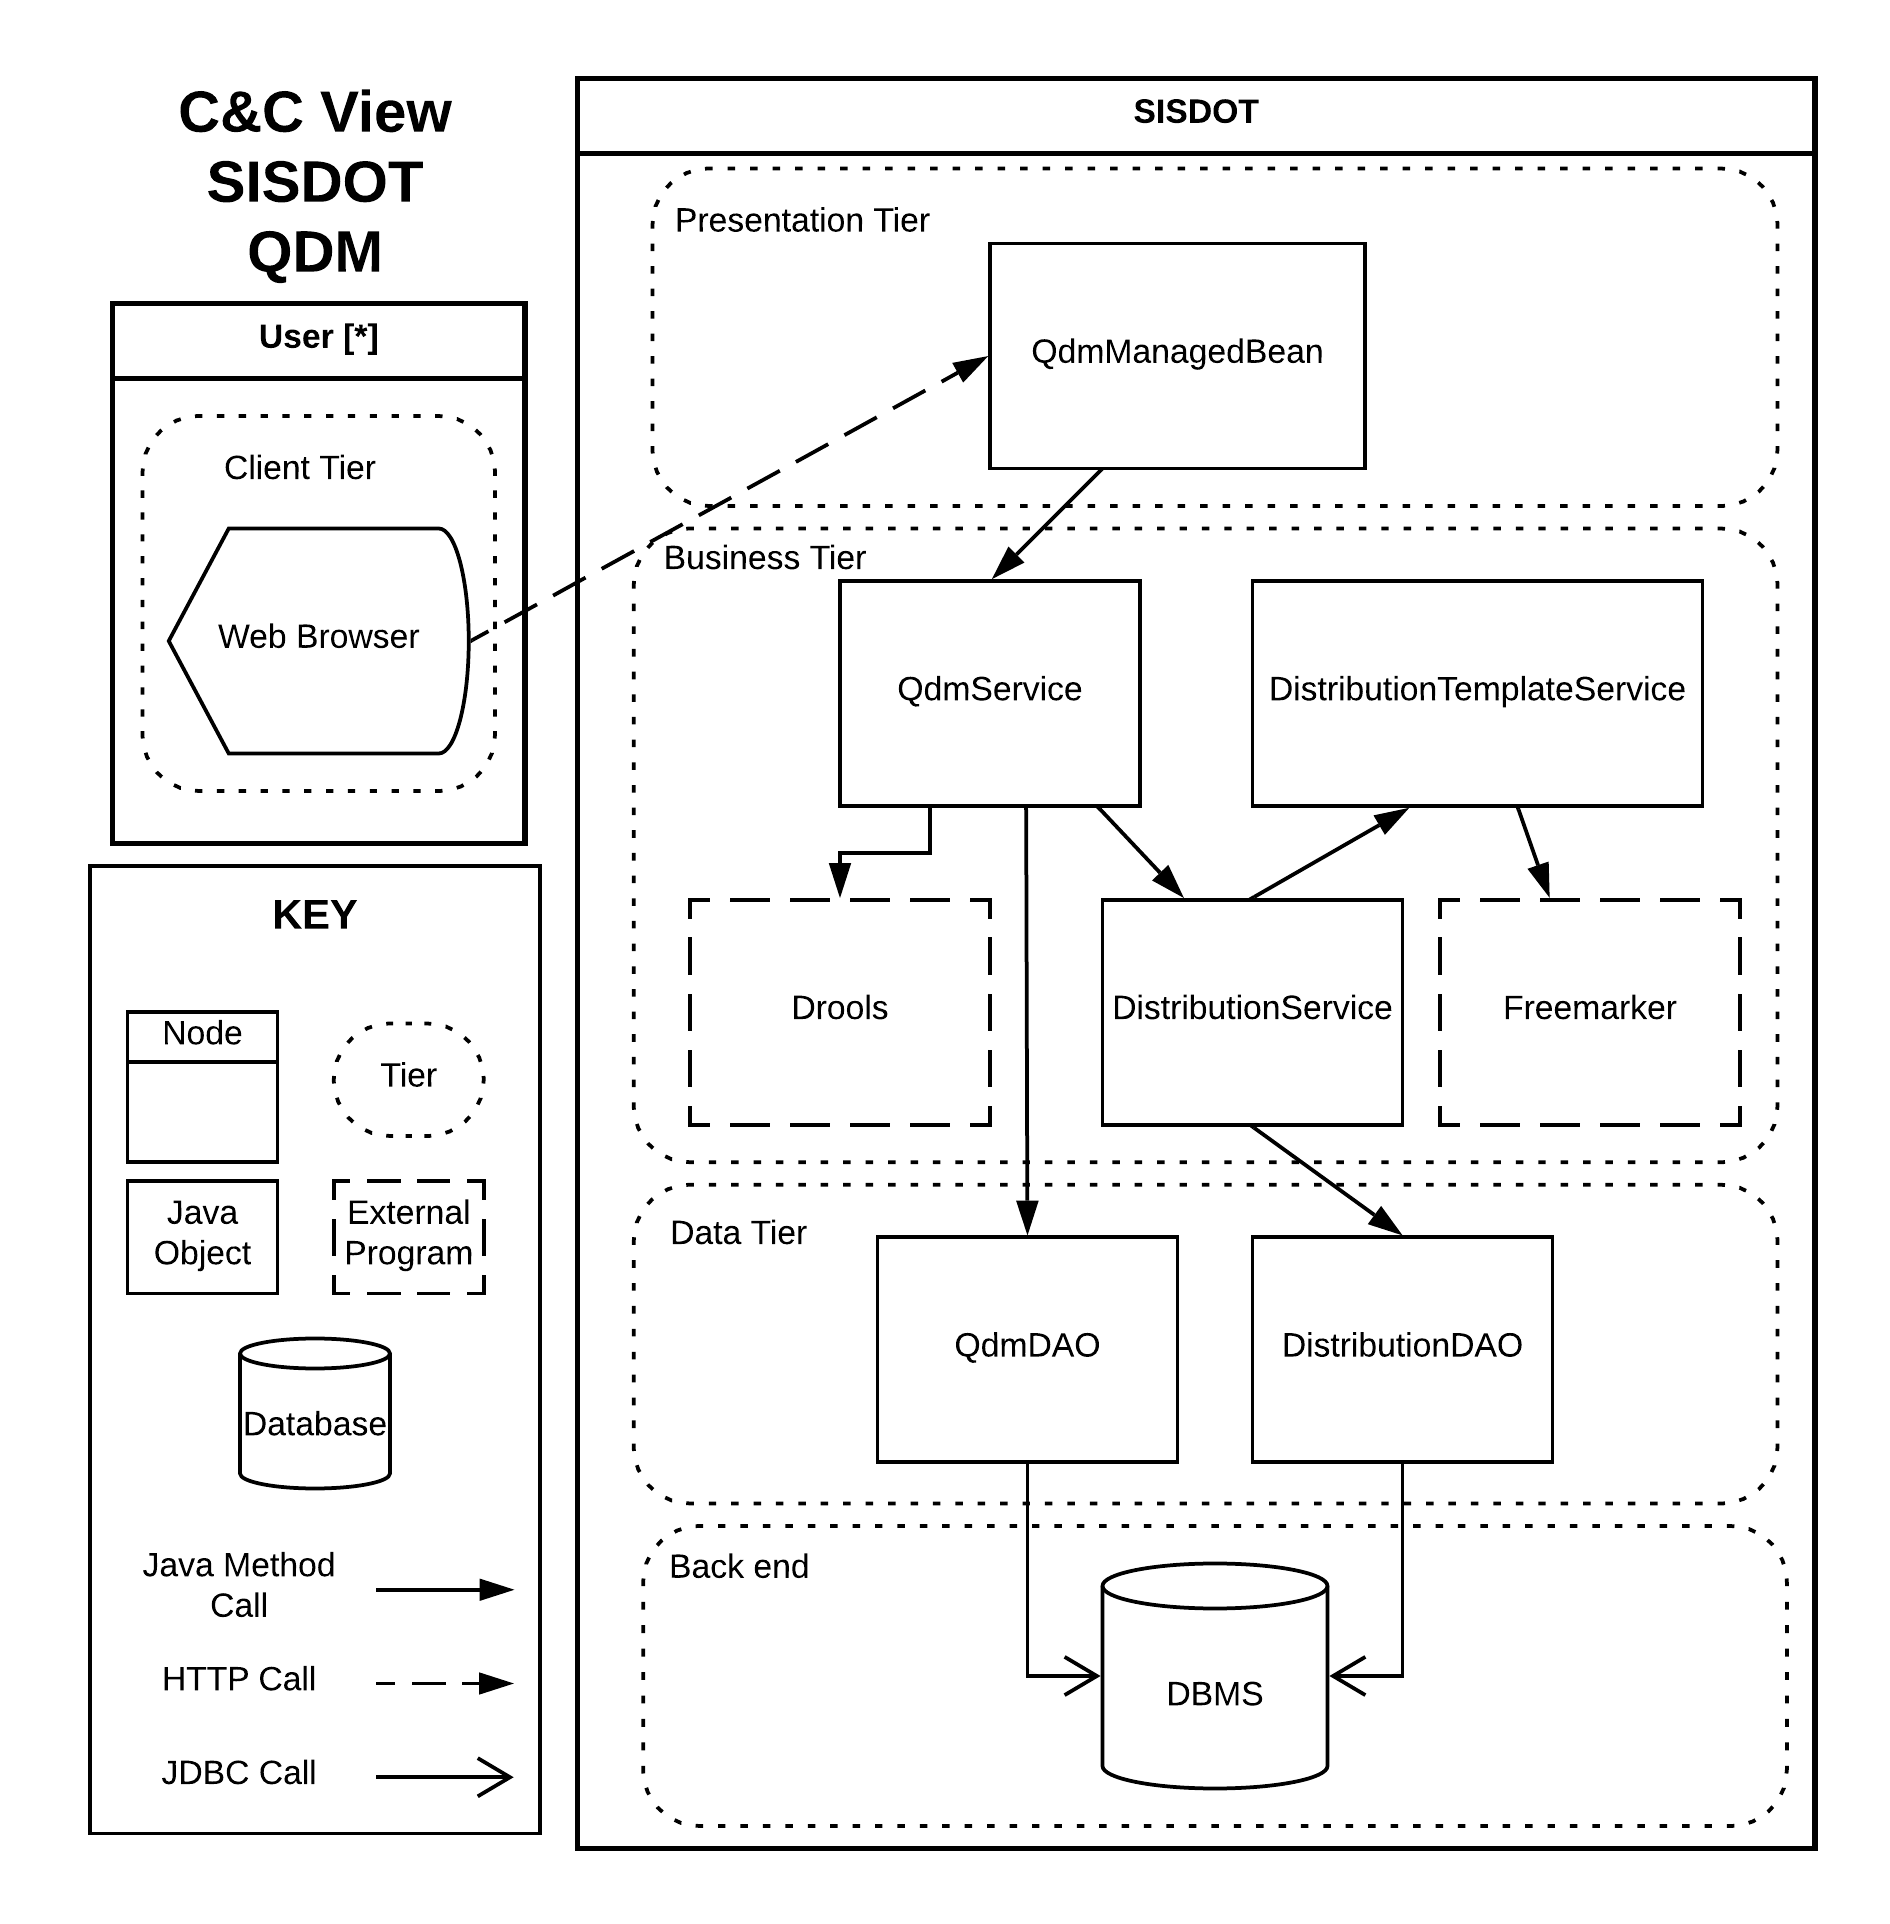
\includegraphics[scale=0.49]{img/runtimeView_qdm.png}
	\caption{Runtime view of the architecture} 
	\label{fig:runtime_qdm}
\end{figure}

\textcolor{red}{arrumar exemplo mais completo de DRL}

\textcolor{red}{falar sobre as regioes da DRL? (qc, fracao, cargo)}

\begin{lstlisting}[frame=single, float=*t, language=DRL, caption=Example of a \emph{low-level Drools rule}, label={code:drl}]
rule "HLR 1"   	
  when
    $qc: QuadroDeCargosVO( 
       (operational == OPERATIONAL || operational == NOT_OPERATIONAL)
       , natureId not in (50, 51)
       , valueId in (23, 41, 90, 50, 42, 31, 21, 32, 20, 30, 40) 
    )	
    $roles: List( size > 0 ) from accumulate ( 
      $dep: DepartmentVO(
         depId not in (14086, 1130)
      ) from $qc.deps 
      and
      $role: RoleVO(
         function == "ROLE"
         , roleId not in (364, 539, 121, 2205, 528, 2204, 539) 
         , rankId in (24, 23, 44, 22, 42) 
         , armsId not in (1055, 10, 833, 5308, 5393, 729, 5110, 15, 5112, 5390, 12) 
      ) from $dep.roles 
      and  		
      QualificationVO(
         code not in ("782", "756", "793", "768", "765", "751", "921", "749", "767", "748")
      ) from $role.qualifications
      and
      ObservationVO(
         code in ("40D","40K")
      ) from $role.observations;
	
      collectList( $role )
    )	 		
  then		 
    for(int i=0; i < $roles.size(); i++){       	
      RoleVO c = (RoleVO) $roles.get(i);
      helper.add(1051000007, c.getDepartmentId(), c.getRoleId());
    }
end
\end{lstlisting}

\emph{Considering the user interaction}, a previously authenticated specialist on the distribution of equipment throughout the Brazilian Army, using her web browser, requests the web page that allows the generation of QDMs (one of the main products of SISDOT). 
After selecting the \emph{generic organizational unity} for which a QDM would be generated, the system sends a request to the server. The client tier is responsible for these actions. The request is then received by a component of the presentation tier, more specifically by a \emph{managed bean} that works as a \emph{front controller} (in this case, a JSF controller). 

This controller validates the request data, before sending a new request to the business tier. In the business tier, the service 
that implements the business rules related to the QDM domain object is invoked to start the QDM generation process, which includes actions to (a) transform \callers into the \emph{low-level rules} specified using the Drools Rule Language (DRL), (b) execute these rules to instantiate a business object that represents a QDM, and (c) save this object in the persistence layer (a relational database). 

This process for generating a QDM starts by retrieving a list of previously registered \callers. An \shc, regardless of its type (either based on the full structure of the organization or based on its components), is related to one or more \emph{military materials / equipment} (MEMs) and defines the respective amount that should be assigned to a military unit (which ranges from an organization, a center, a department, a brigade, or even a military function or qualification of a soldier). 

A high-level rule has one or more distribution rules. Each rule has a type, a value, and an associated description. For example, a rule for a department type has the value of the department identifier and the description of the department name. For a better use of the database, avoiding the definition of numerous columns that would inevitably be null for several rule types, we decided to persist the distribution rules of an \shc using JSON (JavaScript Object Notation), which is converted back to an object when it is retrieved. The set of these rules defines exactly who should receive the MEMs specified by the \shc.

One of the factors that motivated the use of a rule based engine was the similarity between \callers and the ``if-then'' rules of these mechanisms.  %whose essential structure is shown in Listing~\ref{code:drlStructure}.
An \shc has a set of conditions that fits the conditional part of a rule (``if'') and has a set of actions (``then'') that, in this case, trigger the distribution of MEMs throughout the expected military unities.

%\begin{lstlisting}[frame=single, caption={Structure of a rule specified in Drools}, label={code:drlStructure}]
%rule "name"
%    attributes
%    when
%        LHS
%    then
%        RHS
%end
%\end{lstlisting}


The list of retrieved \callers contains only Java objects. In order to be able to use the rule engine in a transparent way for the end users (and also for developers in future maintenance scenarios), we decided to use a meta-programming approach, translating these objects into a set of rules (a program in logic programming) that might be used by a rule-based engine. As mentioned before, we decided to use the \emph{Drools rule-based engine} in the context of SISDOT (Figure \ref{fig:runtime_qdm}), mostly because of its integration capabilities with both JEE systems and the Wildfly application server. Accordingly, the \callers are translated into DRL rules (Listing~\ref{code:drl} presents an example of a \emph{low-level Drools rule}). To this end, we use a template engine (FreeMaker) to implement this particular transformation (Figure \ref{fig:runtime_qdm}), using a template that contains the required \emph{markups} for transforming \shc into \emph{low-level} Drools rules. That is, for each \shc, the template engine populates the template, resulting in a DRL rule consistent with the converted \shc.
% A code snippet of the template used for DRL generation can be seen in Appendix A. 

The RHS of the Drools rule of Listing~\ref{code:drl} iterates over all selected military roles (that satisfy the constraints of the LHS). We use a helper class to assign the equipment id (in this case a \emph{rifle} whose id is 1051000007) to the individual roles. Besides providing means to populate a QDM, this helper class also checks some constraints related to the QDM domain model. 

%\begin{figure}[!ht] \centering
%	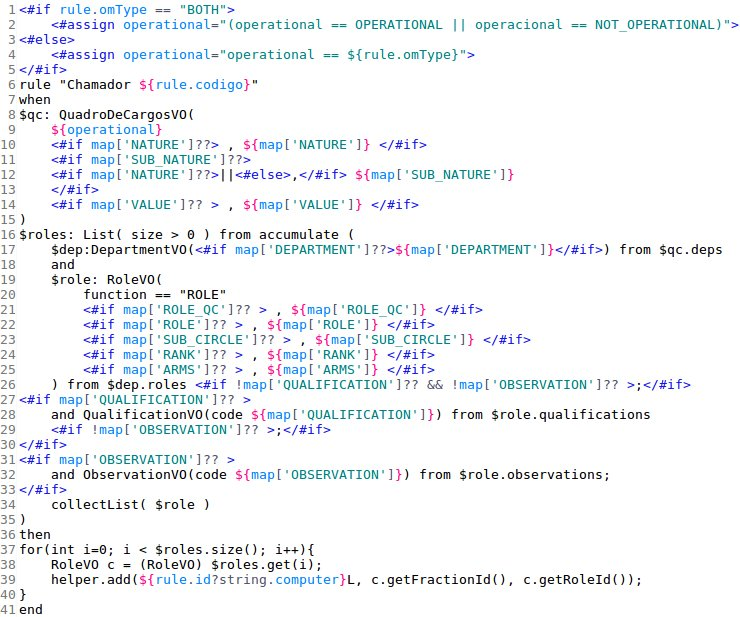
\includegraphics[width=.48\textwidth]{img/artigo_template.jpg}
%	\caption{\it Freemarker template for generating DRL} 
%	\label{fig:template}
%\end{figure}


A QDM is generated for a generic organizational unity (hereafter QC, from \emph{Quadro de Cargos} in Portuguese), selected by the user on the client tier. Therefore, the user-specified QC must be retrieved from the Brazilian Army's enterprise database through a specific Data Access Object (DAO) in the data tier~\cite{alur2003}. From the list of DRL rules, created based on existing \callers, the rule engine is instantiated and these rules are compiled, so that they can be triggered by Drools. The QC domain object is then inserted into the working memory as a fact, an information that is always considered true. The rules are only executed when their conditions are satisfied, based on the specified QC organizational structure. When a rule is valid, that is, it has been activated and the \emph{Left Hand Side} (LHS) conditions are valid, the QDM is populated with the MEMs specified in the \emph{Right Hand Side} (RHS) of the rules. Therefore, we generate a complete QDM object after verifying all valid rules (previously registered in the database) for the selected QC. 

After generating a QDM domain object, it is saved on the database and we let the domain expert know of the success of the operation using a simple user interface message. The domain expert can then perform the necessary operations on the generated QDM, including a workflow involving  its edition, homologation, and validation.  



%%%%%%%%%%%%%%%%%%%%%%%%%%%%%%
%% A Domain Specific Language for testing QDM Generation
%%%%%%%%%%%%%%%%%%%%%%%%%%%%%%
\subsection{A Domain Specific Language for testing QDM Generation}

As explained before, to generate a QDM, a set of \callers must be previously declared. This is a time-consuming task, particularly when using the interface of the system. In order to facilitate the definition of the \callers used in the automated test scripts, we decided to implement \hlrdsl---a DSL (Domain Specific Language) that enables us to specify \callers in a clear, objective, and declarative way (and most important, without using the interface of the SISDOT system). 

We implemented \hlrdsl  using Xtext, which generates plugins that allow code editing in both Eclipse and IntelliJ, plus an editor that can be embedded in a web application. This way, a developer writing test scripts might use \hlrdsl to take advantages of the functionality provided by these plugins. To implement a DSL using Xtext, it is first necessary to declare a grammar expressed using a syntax similar to ANTLR~\cite{parr2013}. Listing~\ref{code:gramatica} presents the grammar of our DSL. From this grammar,the Xtext tool suite generates a lexer, a parser, a set of classes representing the AST (Abstract Syntax Tree), and an editor with several features typically available in IDEs.
% Although Xtext provides an interesting implementation for all these concerns, a language designer is also able to customize several of the Xtext outcomes~\cite{bettini2016}.


\begin{lstlisting}[frame=single, language=Xtext, caption={\it Xtext grammar defining the DSL structure}, label={code:gramatica}]
grammar br.unb.cic.sisdot.chamador.HLRDsl 
with org.eclipse.xtext.common.Terminals
generate hlrdsl "http://www.unb.br/sisdot/hlrdsl"

Model:
rules += Rule*;

Rule:
'rule' code = INT '{'
('type' '=' type=OmType ',')?
'materials' '=' '['items+=Item (',' items+=Item)*'],'
'cnds' '=' '['cnds+=Condition (',' cnds+=Condition)*']'
'}';

Item: '(' codot=STRING (':' name=STRING)? ':' amount=INT ')';

Condition:
'(' ('cond' '=' cond=ConditionType ',')?
'type' '=' type = RuleType ','
'values' '=' '[' values+=STRING (',' values+=STRING)* ']'
')';

enum OmType: BOTH | OPERATIONAL | NOT_OPERATIONAL;
enum ConditionType: AFF | NEG;
enum RuleType: NATURE | SUB_NATURE | VALUE | DEPARTMENT | ARMS | ROLE_QC | SUB_CIRCLE | RANK | ROLE | QUALIFICATION | OBSERVATION ;
\end{lstlisting}

Listing \ref{code:dslExample} presents a simple example of a \shc declaration using our DSL. The goal of this rule is to distribute 
the materials (defined in the list of materials construct) for \emph{operational} OMs (see the type construct) and militaries \emph{not working in the specified list of departments} with a set of qualifications and roles. \textcolor{red}{While the definition of this rule using our DSL requires 12 lines of code, the corresponding definition of the same rule using a Java test case requires more than 50 lines of imperative code.}

\begin{small}
	\begin{lstlisting}[frame=single, language=DSL, caption={\it Example of a \shc declaration using our DSL}, label={code:dslExample}]
rule 1 { 
    type = OPERATIONAL, 
    materials = [ 
        ("1051000007" : "Rifle" : 1), 
        ("1020100011" : "Rifle Carrying Case" : 2)
    ], 
    cnds = [ 
        (cond=NEG, type=DEPARTMENT, values=[14086 , 1130]),
        (type=QUALIFICATION, values=[782, 756]), 
        (type=ROLE, values=[2, 12, 15, 21])
    ]
}
	\end{lstlisting}
\end{small}

Our first test approach consists first in the specification of the required \callers in a \hlrdsl file. Next, the \emph{behavior under test} is detailed as features using the Cucumber~\cite{wynne2017cucumber} framework (we present an example of a feature in Listing \ref{code:cucumber}). After that, the developer details the implementation steps of the features by (a) specifying which \callers(previously declared using our DSL) should be considered in the test execution, (b) specifying which QC the QDM should be generated, and (c) specifying the expected results in terms of the properties of the expected QDM. To this typical scenario, we use a testing  infrastructure that supports several facilities, that aims to increase productivity, such as: database connectivity, auxiliary methods for executing queries in the database, and predeclared rules in the rule engine.

That is, \hlrdsl simplifies the process of specifying \callers and its primary goal was to assist in test activities. However, after presenting to domain experts some examples of \callers specified using our DSL, we realized that \hlrdsl might also be useful to simulate the specification of rules, allowing a better understanding of the effect of each \shc for building QDMs.

\begin{lstlisting}[frame=single, language=Cucumber, caption={\it Cucumber feature}, label={code:cucumber}]
Feature: QDM 757311
As a user
I want to generate a QDM from HLRs

Scenario: Test 1
Given QC with code 757311
And HRL: 1, 2
When I generate a QDM
And the results are consistent
Then positions must be populated
| idDep    | idPos   | codot      | amount |
| 6765748  | 10403   | 1051000025 | 1      |
| 6765748  | 10403   | 1020100017 | 1      |
| 6765748  | 10403   | 1020100013 | 1      |
| 6765748  | 10403   | 1051000006 | 1      |
| 6765748  | 21328   | 1051000025 | 1      |
| 6765750  | 10122   | 1051000025 | 1      |    
| 6765793  | 13276   | 1051000025 | 6      |
| 6765796  | 24655   | 1051000025 | 1      |
| 6765796  | 24429   | 1051000025 | 2      |
| 6765798  | 24429   | 1051000025 | 3      |
| 6765798  | 11433   | 1051000025 | 9      |   
And the final result must be:
| codot      | amount |
| 1020100013 | 74     |
| 1020100017 | 74     |
| 1051000006 | 74     |
| 1051000025 | 74     |

\end{lstlisting}

Our second test approach automatically generates test cases from our DSL and from a random sample of simple combinations that characterize artificial organizational unities. This \emph{property based approach} involves a custom Maven plugin that currently generates simple test cases, freeing the tester to create only complex tests related to the QDM generation. 

\textcolor{red}{These test cases are generated from a combination of conditions, for example: one test case only for operational OMs and another for non-operational OMs; a test case for the different kinds of OMs (artillery, infantry, cavalry, aviation and helicopters, general services, and so on), combining with the operational type, such as: operational infantry OMs and non-operational infantry OMs. These combinations are generated for simple cases so that they are easy to verify without the need to manually implement Java test scripts for generating QDMs.}

% O Maven plugin desenvolvido define diversos cenários que serão gerados para cada QC declarado. Cada cenário é responsável pela geração de uma high-level rules no formato DSL e um arquivo de definição do cenário no formato do cucumber. Para cada cenário é gerado um QDM para o QC, usando a high-level rule gerado e o resultado deste QDM é conferido de acordo com os dados previstos na definição do cenário do cucumber. Foram criadas diversas combinações de cenários e para cada uma delas alguns dos valores das propriedades são gerados randomicamente, seguindo a técnica PBT. 

The Maven plugin developed defines several scenarios that will be generated for each declared QC. Each scenario is responsible for generating a high-level rules in DSL format and a scenario definition file in cucumber format. For each scenario, a QDM for the QC is generated, using the generated high-level rule and the result of this QDM is checked according to the predicted data in the cucumber scenario definition. Several combinations of scenarios have been created and for each of them some of the values of the properties are generated randomly, following the PBT technique.

% Os cenários de teste foram divididos em três grupos, de acordo com as seções da DRL (QC, fração e cargo). Isso foi feito pois cada região é testada de forma quase que independente, possuindo dependência apenas da validade da região anterior. Por exemplo: a região de fração só é avaliada se a região de QC tiver sido avaliada como verdadeira, então essas regiões podem ser testadas de forma independente ao assumir que a região anterior é verdadeira e que foram gerados casos de testes que ajudaram a validar o funcionamento das condições da região anterior. Ao assumir a independência dos grupos, para fins de teste, é possível focar nas combinações das propriedades de cada grupo, facilitando a geração de cenários de teste. 

The test scenarios were divided into three groups, according to the sections of the DRL (QC, fraction and charge). This was done because each region is tested almost independently, having dependence only on the validity of the anterior region. For example: the fraction region is evaluated only if the QC region has been evaluated as true, then these regions can be tested independently by assuming that the previous region is true and that test cases have been generated which have helped to validate the conditions of the previous region. By assuming the independence of the groups, for testing purposes, it is possible to focus on the combinations of the properties of each group, facilitating the generation of test scenarios.

% Cada grupo de cenários é responsável por testar várias das combinações das propriedades da entidade relativa ao grupo (QC, fração ou cargo). Em cada cenário é definido uma high-level rule e uma lista com os resultados esperados, que são gerados de acordo com a combinação específica de propriedades deste cenário. Como o MEM definido na high-level rule não interfere na execução das regras, foi definido um MEM padrão para todas as high-level rules geradas, assim como a quantidade igual a um (unitário). Isso foi feito para diminuir a complexidade do algoritmo de geração ao não precisar acessar o banco de dados várias vezes para recuperar MEMs de forma randômica, tendo em vista que não interferem na avaliação das regras envolvidas na geração do QDM.

Each scenario group is responsible for testing various combinations of entity properties relative to the group (QC, fraction or charge). In each scenario a high-level rule and a list with the expected results are defined, which are generated according to the specific combination of properties in this scenario. Since the MEM defined in the high-level rule does not interfere in the execution of the rules, a standard MEM has been defined for all high-level rules generated, as well as a quantity equal to one (unitary). This was done to reduce the complexity of the generation algorithm by not having to access the database several times to retrieve MEMs in a random way, since they do not interfere in the evaluation of the rules involved in the generation of QDM.

% No grupo de QC existem as seguintes propriedades: operacionalidade, natureza, subnatureza e valor. Foram criados cenários específicos para cada propriedade e para combinações entre elas. Para a propriedade natureza do QC, por exemplo, foram definidos os seguintes cenários:

In the QC group there are the following properties: operability, nature, sub-nature and value. Specific scenarios have been created for each property and for combinations between them. For the nature property of the QC, for example, the following scenarios have been defined:

\begin{itemize}

% \item natureza válida e tipoOM válido: este cenário gera um QDM válido, com resultados válidos, pois neste cenário é criado um high-level rule com os mesmos valores de natureza e operacionalidade (tipoOM) do QC para o qual será gerado o QDM, ou seja, natureza e tipoOM válidos;

\item valid nature and valid typeOM: this scenario generates a valid QDM, with valid results, because in this scenario a high-level rule with the same values of nature and operability (typeOM) of the QC for which the QDM is generated is created , valid nature and typeOM;

% \item natureza válida e tipoOM válido (AMBOS): este cenário funciona de forma parecida com o anterior, mas o tipoOM é definido como "AMBOS" no high-level rule. Este tipoOM indica que o QC pode ser operacional ou não-operacional;

\item valid type and valid typeOM (BOTH): this scenario works similarly to the previous one, but the typeOM is set to "BOTH" in the high-level rule. This type indicates that QC can be operational or non-operational;

% \item natureza válida e tipoOM inválido: o valor da natureza é o mesmo do QC, pois é válido, e o valor do tipoOM é alterado. Por exemplo: se o QC for operacional o valor é alterado para não-operacional e vice-versa;

\item valid nature and invalid typeOM: the value of nature is the same as the QC, since it is valid, and the value of typeOM is changed. For example: if the QC is operational the value is changed to non-operational and vice versa;

% \item natureza inválida e tipoOM válido: o valor da natureza deve ser inválido no high-level rule, ou seja, um valor diferente da natureza do QC. A geração deste valor inválido de natureza é realizado de forma randômica, usando a seed configurada no plugin maven, em uma lista de códigos de naturezas reais previamente definida;

\item Invalid nature and valid typeOM: Nature value must be invalid at high-level rule, i.e., a value different from the nature of QC. The generation of this invalid value of nature is performed in a random fashion, using the seed configured in the maven plugin, in a previously defined real-life code list;

% \item natureza inválida e tipoOM inválido: os valores de natureza e tipoOM são inválidos, e são gerados conforme citado anteriormente: invertendo o valor de operacionalidade e recuperando randomicamente um código de natureza da lista declarada previamente;

\item Invalid nature and invalid typeOM: the values of nature and typeOM are invalid, and are generated as previously mentioned: reversing the value of operability and randomly retrieving a code of nature from the list previously declared;

% \item negar natureza, inválido: as combinações citadas anteriormente nesta lista possuem high-level rules com regras do tipo "AFIRMACAO", o tipo padrão de uma regra. Mas existe o tipo "NEGACAO", onde a regra é negada, ou seja, a condição (na DRL) é válida quando o valor testado não pertence à lista de valores especificados na regra. Neste cenário, por exemplo, há uma regra de negação da natureza de forma que o QDM seja inválido. Então foi criada uma regra para "NATUREZA" do tipo "NEGACAO" definindo como valor o código da natureza do QC. Com isso, esta regra não é válida para este QC, sendo válida para todas as outras naturezas exceto a deste QC;

\item deny nature, invalid: the combinations previously mentioned in this list have high-level rules with rules of type "AFFIRMATION", the standard type of a rule. But there is the type "DENIAL", where the rule is denied, that is, the condition (in the DRL) is valid when the value tested does not belong to the list of values specified in the rule. In this scenario, for example, there is a nature negation rule so that QDM is invalid. Then a rule for "NATURE" of the type "DENIAL" was created defining the code of the nature of QC. Therefore, this rule is not valid for this QC, being valid for all other natures except that of this QC;

% \item negar natureza, válido: para este cenário é criado uma high-level rule com uma regra para "NATUREZA" do tipo "NEGACAO", mas gerando um código de natureza diferente da natureza do QC. Com isso, esta regra é válida para este QC.

\item deny nature, valid: for this scenario a high-level rule with a rule for "NATURE" of type "DENIAL" is created, but generating a code of a nature different from the nature of QC. Therefore, this rule is valid for this QC.
\end{itemize}

% Seguindo a mesma linha de combinações utilizadas paras cenários envolvendo natureza do QC, foram criados cenários para subnatureza e valor. Não foram criados cenários para tipoOM pois esta é uma propriedade de preenchimento obrigatório no high-level rule e a checagem de sua validade já é exercitada em todos os cenários do grupo. Na Table \ref{table:valor} são apresentados os cenários definidos para o Valor do QC e suas combinações. Na primeira coluna é apresentado o número do cenário, criado apenas para facilitar uma possível referência a uma linha específica da tabela. As outras colunas contém os valores das propriedades do QC sendo combinadas. A células com valor 0 indicam que o valor desta propriedade, indicada pela coluna, é inválido, ou seja, deverá ser selecionado um valor randomicamente de uma lista previamente definida e este valor deve ser diferente do valor que essa propriedade apresenta no QC. As células com o valor 1 indicam que o valor desta propriedade é válido, ou seja, é o mesmo valor definido no QC para esta propriedade. As células sem valor indicam que essa propriedade não faz parte da combinação. 

Following the same line of combinations used for scenarios involving the nature of QC, scenarios were created for sub-nature and value. No scenarios have been created for typeOM because this is a mandatory property in the high-level rule and checking its validity is already exercised in all scenarios of the group. In Table \ref{table:valor} the scenarios defined for the Value of QC and its combinations are presented. In the first column the scenario number is displayed, created only to facilitate a possible reference to a specific row in the table. The other columns contain the QC property values being combined. Cells with a value of 0 indicate that the value of this property, indicated by the column, is invalid, that is, a random value must be selected from a previously defined list and this value must be different from the value that this property has in QC. Cells with a value of 1 indicate that the value of this property is valid, that is, it is the same value defined in the QC for this property. Cells with no value indicate that this property is not part of the combination.

\begin{table}[htb!]
	\centering
	\caption{Defined Scenarios for QC Value}
	\label{table:valor}
	\begin{center}
		\begin{tabular}{ccccc}
			\toprule
\textbf{Scenarios} & \textbf{Value} & \textbf{Subnature} & \textbf{Nature} & \textbf{TypeOM} \\ \hline
1                & 0              &                      &                   & 0               \\ \hline
2                & 0              &                      &                   & 1               \\ \hline
3                & 1              &                      &                   & 0               \\ \hline
4                & 1              &                      &                   & 1               \\ \hline
5                & 0              &                      & 0                 & 0               \\ \hline
6                & 0              &                      & 0                 & 1               \\ \hline
7                & 0              &                      & 1                 & 0               \\ \hline
8                & 0              &                      & 1                 & 1               \\ \hline
9                & 1              &                      & 0                 & 0               \\ \hline
10               & 1              &                      & 0                 & 1               \\ \hline
11               & 1              &                      & 1                 & 0               \\ \hline
12               & 1              &                      & 1                 & 1               \\ \hline
13               & 0              & 0                    & 0                 & 0               \\ \hline
14               & 0              & 0                    & 0                 & 1               \\ \hline
15               & 0              & 0                    & 1                 & 0               \\ \hline
16               & 0              & 0                    & 1                 & 1               \\ \hline
17               & 0              & 1                    & 0                 & 0               \\ \hline
18               & 0              & 1                    & 0                 & 1               \\ \hline
19               & 0              & 1                    & 1                 & 0               \\ \hline
20               & 0              & 1                    & 1                 & 1               \\ \hline
21               & 1              & 0                    & 0                 & 0               \\ \hline
22               & 1              & 0                    & 0                 & 1               \\ \hline
23               & 1              & 0                    & 1                 & 0               \\ \hline
24               & 1              & 0                    & 1                 & 1               \\ \hline
25               & 1              & 1                    & 0                 & 0               \\ \hline
26               & 1              & 1                    & 0                 & 1               \\ \hline
27               & 1              & 1                    & 1                 & 0               \\ \hline
28               & 1              & 1                    & 1                 & 0               \\ \hline
		\end{tabular}
	\end{center}
\end{table}

% No grupo Cargo existem as seguintes propriedades: código do cargo, subcírculo ao qual o cargo pertence, o posto (patente) necessário para ocupar o cargo, e a arma (Arma, Quadro ou Serviço) necessária para ocupar o cargo. O subcírculo está relacionado às graduações (posto/patente) existentes, servindo como uma forma de agrupamento. Por exemplo: o subcírculo superior agrupa as patentes de coronel, tenente-coronel e major; o subcírculo subalterno agrupa os tenentes. 

In the Cargo group there are the following properties: position code, sub-circle to which the position belongs, position (patent) needed to fill the position, and the weapon (Weapon, Frame or Service) required to fill the position. The sub-circle is related to existing (rank/patent) grades, serving as a form of grouping. For example: the upper sub-circle groups the patents of colonel, lieutenant-colonel and major; the subordinate sub-circle groups the lieutenants.

% Para cada cenário do grupo de cargos foi selecionado um cargo aleatoriamente da lista de cargos do QC, utilizando a seed configurada no plugin maven. De acordo com o cargo selecionado são geradas as regras conforme a combinação de propriedades especificada para o cenário. Para cada cenário, além das regras, é gerada também uma lista contendo os resultados esperados, ou seja, os dados que se espera encontrar no QDM gerado para o QC. 

For each scenario in the job group, a job was randomly selected from the QC job list, using the seed configured in the maven plugin. According to the selected position, the rules are generated according to the combination of properties specified for the scenario. For each scenario, in addition to the rules, a list containing the expected results is generated, that is, the data expected to be found in the QDM generated for the QC.

% Para este trabalho foram especificados 100 cenários. Todos os cenários gerados, independente do grupo, contém um high-level rule, com as regras referentes à combinação de propriedades definida para o cenário, e uma lista de resultados esperados, que serão comparados com os dados do QDM gerado. Para cada QC declarado no plugin é gerada uma lista de cenários. Para cada QC é gerado um arquivo cucumber contendo os cenários definido para este QC. A geração do arquivo é realizada com o uso do Freemarker, usando um template previamente definido.

For this work 100 scenarios were specified. All generated scenarios, independent of the group, contain a high-level rule, with rules relating to the combination of properties defined for the scenario, and a list of expected results that will be compared with the generated QDM data. For each QC declared in the plugin a list of scenarios is generated. For each QC is generated a cucumber file containing the scenarios defined for this QC. File generation is done using Freemarker, using a predefined template.

% O processo de geração automática de testes pode ser resumido da seguinte maneira: o plugin maven deve ser declarado e configurado, indicando a lista com os códigos dos QCs para os quais devem ser gerados testes. Então, para cada QC da lista são gerados cenários, com variações em suas propriedades de acordo com o QC sendo testado. Os cenários gerados são transformados em arquivos do cucumber e de DSL, que representam os cenários gerados. Houve então uma conversão dos cenários gerados com base na técnica Property-based Testing (PBT) em casos de teste, por exemplo, que serão executados automaticamente durante a fase adequada do ciclo de vida de \textit{build} do maven. Existe a possibilidade de geração de relatório da execução dos testes em alguns formatos, como: html e json.

The automatic test generation process can be summarized as follows: The maven plugin must be declared and configured, indicating the list of QC codes for which tests must be generated. Then, for each QC of the list scenarios are generated, with variations in their properties according to the QC being tested. The generated scenarios are transformed into cucumber and DSL files, which represent the generated scenarios. There was then a conversion of the generated scenarios based on the Property-based Testing (PBT) technique into test cases, for example, that will run automatically during the appropriate maven build phase. There is the possibility of reporting the execution of tests in some formats, such as: html and json.

% \begin{lstlisting}[frame=single, language=Plugin, caption={\it Maven plugin for test generation}, label={code:plugin}]
% <plugin>
%   <groupId>xxx</groupId>
%   <artifactId>xxx</artifactId>
%   <executions>
%     <execution>
%       <id>execute</id>			
%       <configuration>
%         <seed>10</seed>				
%         <qcs>702311,762314,575311</qcs>				
%       </configuration>
%       <goals>
%         <goal>generate</goal>
%       </goals>
%     </execution>
%   </executions>
% </plugin>	
% \end{lstlisting}

\textcolor{red}{In this second approach, for each of the possible combinations, we generate a \shc that meets the conditions and a cucumber feature that exercises the \shc and compares the expected results declared in the feature. Each \shc is considered during the generation of the QDM to the QCs specified in the maven plugin.
That is, to use this architecture characteristic (here we consider testability as an architecture concern), we ``feed'' the maven plugin with a list of QC codes for which the QDMs should be generated, besides other optional information, which have default values, such as: database connection string, seed to be used in the random selection of values within a combination (e.g., considering 20 different kinds of organizational unities, randomly take 5 for generating the set of combinations), and the output directory where the code should be exported. }

After running the plugin, with the generated code, the tests are executed in a similar way to the test definitions detailed before. The tests run along with the other unit tests declared, whether DSL-based or not.





%%%%%%%%%%%%%%%%%%%%%%%%%%%%%%%%%%%%%%%%%%%%%%
%% Empirical Study
%%%%%%%%%%%%%%%%%%%%%%%%%%%%%%%%%%%%%%%%%%%%%%
\section{Empirical Study}
\label{sec:case_study} 
For the validation of the proposed architecture we conducted an empirical study, which consists of the evaluation of the main architectural decisions of SISDOT, which relate to the generation of QDMs. The case study aims to answer the following research questions:

\begin{itemize}
	\item \textbf{RQ.1}: Does our proposed approach, based on meta-programming, generate correct QDMs?
	\item \textbf{RQ.2}: Does the use of a DSL reduce the effort necessary to implement the test cases that target QDM generation? 
	\item \textbf{RQ.3}: Does our proposed approach, based on meta-programming, generate QDMs within a satisfactory time-frame?
\end{itemize}

\textbf{RQ.1} deals with the most important concern: correctness regarding the QDM generation. It is intended to demonstrate that the solution not only automatically generates the rules, eliminating the work that the developer would have to implement the solution in Java, but also that the proposed approach leads to the expected QDMs when considering a well defined set of \callers. \textbf{RQ.2} is related to the productivity of the tester and demonstrates how much code the developer have to write when using our DSL, compared to the effort to specify \callers using the Java language in unit test cases. During the activities of requirements elicitation,we identified a softgoal stating the  acceptable time for generating a QDM, which should not be above 10 seconds, when using 1000 \callers. Thus, \textbf{RQ.3} serves to ensure that the QDMs are generated in a satisfactory time.



%%%%%%%%%%%%%%%%%%%%%%%%%%%%%%
%% Data Collection and Analysis Procedures
%%%%%%%%%%%%%%%%%%%%%%%%%%%%%%
\subsection{Data Collection and Analysis Procedures}

We answer our first question qualitatively using the focus group method. Although this might look like disappointing (under the perspective of more formal methods), we have strong evidences collected from the domain experts that our approach has produced correct QDMs. We believe that this correctness is due to several factors, including the involvement of the domain experts that helped us to full understand the requirements and the expertise of our development team. Nevertheless, the decision of not writing the low-level rules at the source code level, but instead using a program generation approach that has reduced significantly the effort needed to \emph{hand write} those rules, has also contributed to achieve this confidence about correctness. 

We use a quantitative approach to answer the other two research questions.
To this end, we collected two metrics: lines of code (LOC) and execution time. The choice of these two metrics is related to the size of the code, which may indicate higher productivity; and to the fulfillment of the functional requirement that determines the maximum execution time for QDM generation. 

\textcolor{red}{arrumar: nao sao 66
In the quantitative assessment, we use as a benchmark 200 \callers. These \callers correspond to real rules used by the Brazilian Army to perform some tests related to the generation of QDMs.} We converted each \shc written using JUnit to their correspondent one specified using our DSL.

Foram utilizados 200 chamadores, sendo que 100 deles são do tipo ABAS (Estrutura Organizacional por Componentes) e correspondem a chamadores reais utilizados pelo Exército Brasileiro (EB), e serviram para a realização de alguns testes na geração de QDMs pela equipe de desenvolvimento. Foram gerados, de forma automática, 100 chamadores do tipo ÁRVORE (Estrutura Organizacional Completa), para que os dois tipos de chamadores fossem contemplados na realização dos testes.

{\color{red}rbonifacio:
  seria possivel explorar algo como cobertura de codigo aqui? ou
  explorar alguma coisa da abordagem PBT? Talvez, usando essa informacao,
  fosse possivel responder a primeira questao de pesquisa usando tanto uma
abordagem qualitativa quanto uma abordagem quantitativa.}

\subsection{Results of the Qualitative Assessment}

% Para responder a primeira questão de pesquisa nós realizamos um grupo focal com os especialistas do negócio com o objetivo de verificar se os QDMs estavam sendo gerado corretamente pelo sistema e na percepção dos usuários.

To answer the first research question we held a focus group with the business experts in order to verify that the QDMs were being generated correctly by the system and in the users' perception.

Focus groups are carefully planned discussions, designed to obtain the perceptions of the group members on a defined area of interest. There are typically between 3 to 12 participants and the discussion is guided and facilitated by a moderator, who follows a predefined structure so that the discussion stays focused. The members are selected based on their individual characteristics as related to the session topic \cite{kontio2004using}. 

% O grupo focal foi conduzido em três etapas. Na primeira etapa (\emph{defining the research problem}) o objetivo do grupo focal foi definido como o nosso interesse em verificar se a abordagem proposta produzia QDMs corretamente e como os usuários estavam verificando essa corretude. Na segunda etapa (participant selection) foi definido o perfil dos participantes: integrantes da equipe responsável por gerar os QDMs para as organizações militares do Exército Brasileiro. Tais participantes compreendem os principais stakeholders e potenciais usuários finais do SISDOT. Quatro participantes dessa equipe foram selecionados, sendo que todos possuem conhecimento necessário para verificar se o quadro de distribuição de materiais foi realizado corretamente, de acordo com o esperado para cada organização militar, com seu respectivo quantitativo de materiais e cargos.

The focus group was conducted in three stages. In the first stage (defining the research problem) the focal group objective was defined as our interest in verifying that the proposed approach produced QDMs correctly and how users were verifying its correctness. In the second stage (participant selection) the profile of the participants was defined: members of the team responsible for generating the QDMs for the military organizations of the Brazilian Army. Such participants comprise the key stakeholders and potential end users of SISDOT. Four participants of this team were selected, all of whom have the necessary knowledge to verify that the material distribution chart was correctly executed, according to what was expected for each military organization, with its respective quantity of materials and positions.

% Na terceira etapa (executing the focus group session) foi realizada o levantamento das informações com o uso grupo focal, que teve duração de 02 horas e meia e foi realizado nas dependências da 4a. subchefia, responsável pela geração dos QDMs e execução do SISDOT. O grupo focal foi conduzido e gerenciado por dois participantes do projeto, o responsável pelo levantamento dos requisitos e pelo arquiteto responsável pelo desenvolvimento da solução disponibilizada. Inicialmente, foi realizada uma explicação pelo time do projeto sobre os objetivos da realização do grupo focal e quais as expectativas da sua execução. Além disso, foram realizadas perguntas direcionadas aos participantes pelos moderadores. O papel dos dois moderadores foi conduzir as questões e fazer com que os participantes especialistas do negócio descrevessem como as atividades estavam sendo realizadas e verificada a sua conformidade. 

In the third stage (executing the focus group session), the information was collected with the use of the focal group, which lasted for 2 hours and a half and was performed in the 4a. sub-boss, responsible for generating the QDMs and executing the SISDOT. The focus group was led and managed by two project participants, the survey leader and the architect responsible for developing the solution. Initially, an explanation was made by the project team about the objectives of the focus group and what the expectations of its implementation are. In addition, questions were directed to the participants by the moderators. The role of the two moderators was to lead the issues and get the business experts to describe how the activities were being carried out and to verify their compliance.

% Analysis. The focus group session result was documented in the note used during the session and in the audio recording used during the session. Todos os participantes relataram terem executado a funcionalidade de geração de QDMs diversas vezes. \emph{Foi reportado que em nenhuma das execuções levou a uma inconsistência}. Além disso, durante a execução do grupo focal o Major responsável pela 4ª Chefia fez questão de gerar um QDM e nos mostrar como era feita a verificação de conformidade, que segue uma estratégia em pares. Tal Major solicitou ao outro participante para verificar no quadro de cargos qual o quantitativo da OM verificada (AMAN), que é uma das OMs mais complexas em termos de cargos e de materiais necessários para que sejam realizadas as suas atividades militares. O quantitativo desejado e esperado de materiais foi devidamente registrado na geração do QDMs pelos chamadores utilizados para essa geração. Demonstrando assim a geração correta da funcionalidade.

Analysis. The focus group session result was documented in the note used during the session and in the audio recording used during the session. All participants reported performing the QDM generation feature several times. \emph{It was reported that in none of the executions has led to an inconsistency}. Furthermore, during the execution of the focus group the Major responsible for the 4ª Chief made a point of generating a QDM and showing us how the compliance check was carried out, following a strategy in pairs. The Major asked the other participant to verify on the table of positions the amount of verified OM (AMAN), which is one of the most complex OMs in terms of positions and materials needed to carry out their military activities. The desired and expected quantity of materials was duly recorded in the generation of QDMs by the callers used for this generation. Demonstrating the correct generation of functionality.

% Os participantes evidenciaram que a funcionalidade estava sendo realizada corretamente e que a atividade manual que eles realizavam se tornou prática, rápida e confiável. No final da atividade foi feito um agradecimento por parte do responsável pela chefia, dizendo que n\~{a}o imaginava atingir tão rapidamente o grau de corretude na distribuição dos materiais para as OMs.

Participants evidenced that functionality was being performed correctly and that the manual activity they performed became practical, fast and reliable. At the end of the activity, a word of thanks was expressed by the head of the department, saying that he did not expect him to achieve so quickly the degree of correctness in the distribution of the materials to the OMs.

\subsection{Results of the Quantitative Assessment} 

%%%%%%%%%%%%%%%%#######################

 Table \ref{table:comparacao} presents a sample of the collected data. The first column contains the \shc code, the second column contains the number of lines of code to represent the \shc using our DSL, and the third column contains the number of lines of code to represent the same rule in the Java language.

\begin{table}[htb!]
	\centering
	\caption{Comparing the number of lines of code need to specify test cases using our DSL and Java}
	\label{table:comparacao}
	\begin{center}
		\begin{tabular}{ccccc}
			\toprule
			\textbf{\shc Code} & \textbf{DSL} & \textbf{Java} & \textbf{Difference} & \textbf{\%}   \\ \midrule
1                 & 10           & 26            & 16                 & 62                      \\ 
2                 & 10           & 25            & 15                 & 60                      \\ 
3                 & 10           & 32            & 22                 & 69                      \\ 
4                 & 11           & 52            & 41                 & 79                      \\ 
5                 & 15           & 41            & 26                 & 64                      \\ 
6                 & 9            & 16            & 7                  & 44                      \\ 
7                 & 18           & 21            & 3                  & 15                      \\ 
8                 & 12           & 25            & 13                 & 52                      \\ 
9                 & 9            & 11            & 2                  & 19                      \\ 
10                & 11           & 23            & 12                 & 53                      \\ 
122               & 10           & 48            & 38                 & 80                      \\ 
123               & 8            & 44            & 36                 & 82                      \\ 
124               & 10           & 54            & 44                 & 82                      \\ 
125               & 8            & 39            & 31                 & 80                      \\ 
126               & 12           & 47            & 35                 & 75                      \\ 
127               & 9            & 43            & 34                 & 80                      \\ 
128               & 9            & 39            & 30                 & 77                      \\ 
129               & 9            & 27            & 18                 & 67                      \\ 
130               & 12           & 25            & 13                 & 52                      \\ 
131               & 12           & 45            & 33                 & 74                      \\ \bottomrule
		\end{tabular}
	\end{center}
\end{table}

Regarding the runtime metrics, we collected the data using an Intel(R) Core{TM} i7-4790 processor, with 16GB of RAM, running Ubuntu 16.04.4 LTS 64-bit operating system, with 4.15.0-24-generic kernel. We used 100 QCs, chosen to represent the various OM types, natures, and sub-natures. For each QC, we generated QDMs using random sets of \callers with size: 400, 700, 1000, 1500, 2000. Since there were only 200 \textcolor{red}{real} \callers already declared, larger quantities contain repeated \callers (which in the end will duplicate the data within a given QDM). The selection of \callers was performed at random, but with the same seed, so that the same sets were used in the generation of QDMs for different QCs. Table \ref{table:tempo} shows a sample of the results obtained with the execution. The first column contains the QC code, and the second column contains the time in milliseconds for the generation of the QDMs using the indicated amount of \callers on the respective column header.

\textcolor{red}{pegar tempos da dissertacao, incluir AMAN ... não achei os dados ainda (tive q formatar o computador uns tempos atrás)}

\begin{table}[htb!]
	\centering
	\caption{Time (ms) for generation of QDMs}
	\label{table:tempo}
	\begin{center}
		\begin{tabular}{|l|r|r|r|r|r|}
			\toprule
			\textbf{QC} & \textbf{400} & \textbf{700} & \textbf{1000} & \textbf{1500} & \textbf{2000} \\ \midrule
101410   & 1866      & 3237      & 4846       & 6877       & 9231       \\
206410   & 1875      & 3170      & 4838       & 6975       & 9348       \\
215304   & 2026      & 3358      & 5235       & 6851       & 9416       \\
231303   & 1954      & 3221      & 4931       & 6715       & 9264       \\
300400   & 1903      & 3132      & 4808       & 6858       & 9283       \\
500312   & 1992      & 3495      & 4709       & 6637       & 9213       \\
524311   & 1999      & 3231      & 4991       & 7061       & 9686       \\
609420   & 1895      & 3162      & 4875       & 6905       & 9259       \\
619321   & 1945      & 3269      & 5010       & 6976       & 9163       \\
627320   & 2006      & 3314      & 5081       & 7522       & 9011       \\
656320   & 1868      & 3197      & 5058       & 7086       & 9398       \\
702311   & 2902      & 4301      & \textbf{6185} & 7753       & 10098      \\
710312   & 1996      & 3237      & 4861       & 6728       & 9102       \\
725310   & 1872      & 3104      & 4860       & 6957       & 9190       \\
727310   & 1949      & 3206      & 4722       & 6795       & 9222       \\
757311   & 2084      & 3359      & 5263       & 6960       & 9230       \\
950401   & 1993      & 3235      & 5076       & 7282       & 10060      \\
1108400  & 2048      & 3458      & 4703       & 6727       & 9575       \\
1112401  & 1880      & 3165      & 4837       & 6873       & 9270       \\
5716900  & 1979      & 3423      & \textbf{4662} & 6504       & 9032       \\
7805004  & 1808      & 2979      & 4710       & 6915       & 9287       \\
1470310  & 1861      & 3091      & 4711       & 6824       & 8996       \\
739310   & 1962      & 3096      & 4722       & 6753       & 9032       \\
8204900  & 1841      & 3052      & 4731       & 6907       & 9348       \\
1501402  & 1869      & 3092      & 4784       & 6873       & 9581       \\
6512900  & 1882      & 3161      & 4796       & 6825       & 9691       \\
2522135  & 1890      & 3115      & 4819       & 6928       & 9153       \\
302401   & 1871      & 3080      & 4898       & 6875       & 9272       \\
1115310  & 1857      & 3131      & 4904       & 6891       & 9201       \\
7038901  & 1955      & 3268      & 5026       & 7450       & 9241       \\
6800901  & 1870      & 3138      & 4895       & 6982       & 8975       \\
6993900  & 1861      & 3090      & 4741       & 6793       & 9445       \\
2205400  & 1890      & 3186      & 5038       & 7107       & 9146       \\
7017901  & 1852      & 3061      & 4773       & 6760       & 9201       \\
2587150  & 1854      & 3147      & 5132       & 6902       & 9034       \\
8417000  & 1917      & 3191      & 4892       & 7010       & 9061       \\
903311   & 1910      & 3180      & 4843       & 6950       & 9346       \\
9015002  & 1893      & 3070      & 4783       & 6792       & 8989       \\
5406194  & 1924      & 3124      & 4870       & 6749       & 8955       \\ \bottomrule
		\end{tabular}
	\end{center}
\end{table}

We exported the collected data to the CSV format, so that we could perform a data analysis using the R environment~\cite{crawley2013}. In the data analysis for \textbf{RQ.2}, which compares the number of lines of code between the two distinct approaches for representing \callers, we created two additional columns: \emph{difference}, which measures the difference in the number of lines of code necessary to specify \callers using Java and our DSL; and \emph{percent of reduction}, which indicates how much less code is necessary to specify a \shc using our DSL, when compared to the direct specification in Java code.

\begin{table}[htb!]
	\centering
	\caption{Analysis of DSL and Java comparison data}
	\label{table:analiseComparacao}
	\begin{center}
		\begin{tabular}{lrrrrr}
			\toprule
			& \textbf{Min.}  & \textbf{Median} & \textbf{Mean}  & \textbf{SD}    & \textbf{Max.}  \\ \midrule
DSL         & 7.00  & 9.00   & 9.67  & 2.01  & 18.00  \\ 
Java        & 9.00  & 23.00  & 28.66 & 18.47 & 130.00 \\ 
Difference  & 2.00  & 13.00  & 18.98 & 18.25 & 121.00 \\ 
\%	        & 14.29 & 56.26  & 54.66 & 21.68 & 93.08  \\ \bottomrule
		\end{tabular}
	\end{center}
\end{table}

Table \ref{table:analiseComparacao} presents some descriptive statistics of the collected data, containing the following columns: minimum value, median, mean, standard deviation, and maximum value. There is a strong correlation (0.982) between the lines of code in Java and the \emph{difference} measurements. This correlation can be seen in Figure \ref{fig:correlacao}. It is possible to identify that as the size of the Java code grows, the difference for the representation in DSL also increases.

\textcolor{red}{regerar figuras em ingles}

\begin{figure}[htb!] 
	\centering
	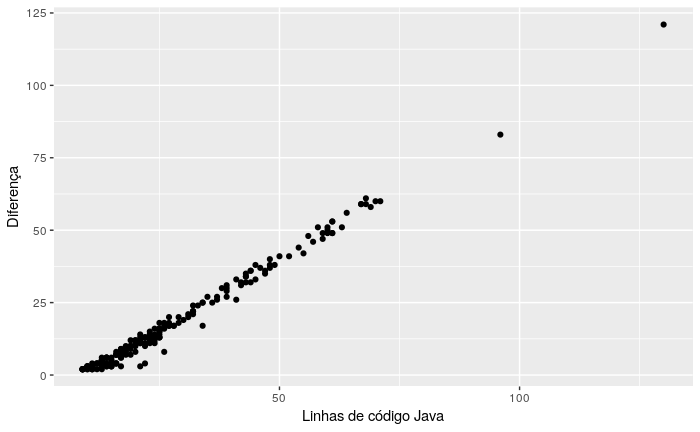
\includegraphics[width=.45\textwidth]
	{img/artigo_correlacao.png}
	\caption{\it Correlation between Java and Difference}
	\label{fig:correlacao}
\end{figure}

Figure \ref{fig:geracao} shows the time necessary to generate QDMs for 5 different QCs. For each of them, 6 QDMS were generated, with different amounts of \callers, 60, 100, 400, 700, 1000 and 2000.

\begin{figure}[!ht] \centering
	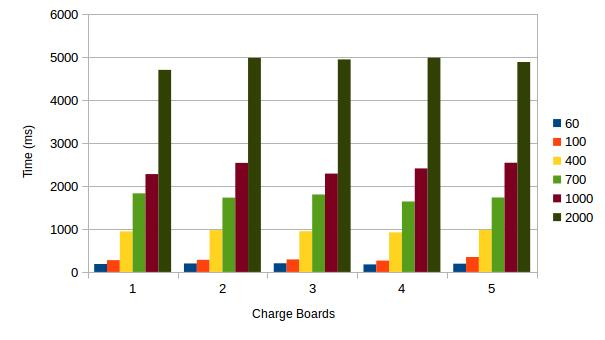
\includegraphics[width=.45\textwidth]
	{img/artigo_geracao.jpg}
	\caption{\it QDM Generation Time (ms)}
	\label{fig:geracao}
\end{figure}



%%%%%%%%%%%%%%%%%%%%%%%%%%%%%%
%% Discussion, Lessons Learned, and Threats to Validity
%%%%%%%%%%%%%%%%%%%%%%%%%%%%%%
\section{Discussion and Threats to Validity}

When analyzing the data related to RQ.2, it was possible to realize that the representation of a \shc using our DSL is on average 45\% smaller than the representation of the same rule in Java. This indicates a possible productivity gain for the developer when writing test cases, since she will have to write a smaller amount of code. In addition, using our DSL, we specify \callers using a declarative approach, which is close to the vocabulary of the problem domain. With respect to the third research question, the limit imposed by the functional requirement of 5 seconds was not exceeded, even when considering 2000 \callers, which is twice the number of \callers expected for the system in production. It is important to notice that these number (5 seconds as time limit and 1000 \callers were collected together with the stakeholders of SISDOT).

The general approach discussed in this paper involves the use of metaprogramming to generate low-level Drools rules from \callers and the use of a DSL to specify \callers during test activities. We have some previous experience using Drools, and, at the beginning of this research collaboration, we realized that the use of a rule based engine (such as Drools), could simplify the computation of QDMs
(one of the main products of SISDOT). Nevertheless, we should try to abstract the use of Drools, mostly due to architectural conformance---we should not introduce new languages during the development of SISDOT. For this reason, we applied a transformational approach, translating Java domain objects into Drools rules at runtime. Perhaps due to the structure of the \callers, the task of implementing this transformational approach was not difficult. We believe that it was the right decision considering the original set of requirements. Surely, a number of uncertainties arise, including: ``will our proposed approach support the expectations of the end-users w.r.t. correctness and time constraints?''. We address this question in our empirical evaluation.

However, we found that testing the process of QDM generation was time consuming, and then we designed a DSL to address the main bottleneck: the specification of \callers either using Java test scripts or the SISDOT user interface (the common way for specifying \callers). Our choice for using Xtext to this end had simplified the entire process for implementing a DSL. Even considering that \hlrdsl is a simple and small DSL, we argue that the set of Xtext tools is really simple and productive, reducing the overall effort to implement the \hlrdsl grammar, parser, and program generator. We could have used other tools and techniques as well, for instance
a metaprogramming approach to support our test activities. However, such approach would not have solved the main problem that motivated us to implement \hlrdsl. In this case, our goal was to design a simple approach for specifying \callers. In the end, \hlrdsl started to be considered an interesting approach for use not only in test activities, but also for simulating QDMs without the need to persist \callers in the production environment. 

Our empirical study presents several limitations. First, we discuss \emph{correctness} based on the results of both integration and acceptance tests, though also considering the opinion of the domain experts that are currently confident that our approach for QDM generation is working properly. Surely, we could have used a more formal approach for discussing correctness, and we postpone this investigation to a future work. Nevertheless, considering the scope of this paper, the feedback from the domain experts and testing outcomes reduce some of ours uncertainties about correctness. 

Second, we only considered 66 real \callers in our study, which served as a basis for measuring the time to generate QDMs. SISDOT is expected to have around 1000 \callers in the production environment. To mitigate the threat related to the small number of available \callers for testing, we considered their repetition when carrying out a performance test of SISDOT. In this way, we expect that the
system would present a behavior similar to the production environment (with respect to performance). The same situation occurs with the comparison of lines of code between the declarations of \callers in DSL and Java. As the number of \callers is relatively small, 
it may not be possible to generalize the results we found.









%%%%%%%%%%%%%%%%%%%%%%%%%%%%%%%%%%%%%%%%%%%%%%
%% Related Work
%%%%%%%%%%%%%%%%%%%%%%%%%%%%%%%%%%%%%%%%%%%%%%
\section{Related Work}
\label{sec:related}

We addressed the main architectural concerns of SISDOT using well-known patterns for enterprise systems~\cite{enterprise-patterns:book} and software architecture patterns ~\cite{pattern-oriented:book}. Moreover, the ideas of using rule based engines to support inference within software systems are also not new~\cite{ORDONEZ2016353,li2012modeling}, and have been particularly explored in the health domain~\cite{mantas2012comparing,li2012modeling,jung2011executing}. For instance, Van Hille et al. present a comparison between Drools and OWL + SWRL for implementing the reasoning procedures of the alert module of an implantable cardioverter defibrillator. The authors conclude that Drools provides greater expressiveness when compared to the other approach. Our decision to use Drools to implement low-level rules was mostly based on its integration to the JEE platform, instead of its expressiveness.
% We also considered the use of Prolog for at least
% expressing the mechanics of the QDM generation, though
% we postponed this work to a future work.

Dingcheng Li and colleagues report on the use of the Drools engine to model and reason about \emph{electronic health records}~\cite{li2012modeling}. To this end, the authors of this mentioned work implemented a \emph{model-to-model translational approach} that converts the specification of phenotyping algorithms expressed using the Quality Data Model (from the National Quality Forum\footnote{http://www.qualityforum.org/Home.aspx}) into Drools rules. Similarly, Jung et al. present an approach for executing medical logic modules expressed in ArdenML using Drools~\cite{jung2011executing}. They also used a model-to-model approach implemented using XSLT. Our approach could also be characterized as being based on \emph{model-to-model transformations}, since we translate a business entity model (represented as the \callers Java domain objects at runtime) into Drools rules, though using FreeMarker as template engine.
% The work of Ostermayer et al. also advocates
% the use of DSLs + template engines to generate Drools
% rules~\cite{toostermayer2013simplifying}.

Several DSLs have been proposed to support test activities. For instance, Mugridge and Cunningham present the \emph{Fit Framework for Integrated Tests}, which is based on a DSL~\cite{Mugridge:2005:FDS:1051337} The Cucumber framework also uses a DSL for expressing the expected behavior of software features~\cite{Wynne:2012:CBB:2331446}. Here, we designed a small DSL to reduce the effort for setting up a suite of acceptance tests (based on Cucumber) for QDM generation, particularly helping the test team to specify \callers. 









%%%%%%%%%%%%%%%%%%%%%%%%%%%%%%%%%%%%%%%%%%%%%%
%% Final Remarks
%%%%%%%%%%%%%%%%%%%%%%%%%%%%%%%%%%%%%%%%%%%%%%
\section{Final Remarks}
\label{sec:conclusao}

In this paper we detailed the main design and architectural decisions we use to implement the mechanisms necessary to support the distribution of materials through the Brazilian Army unities. These decisions included the use of a metaprogramming approach to derive high level business rules in rules specific to a rule based system (Drools) and the definition of a DSL that facilitates the declaration of \callers to build test scripts. 

We carried out an empirical study to validate the proposed architecture, based on the evaluation of one of the main scenarios of our logistic system (SISDOT), related to the generation of QDMs. From the results obtained, it was possible to observe a reduction in the average number of lines of code required for the declaration of a \callers using our DSL, in comparison with the representation of the same \shc in Java. Another result of the case study shows that our approach fulfills a non functional requirement that constraints the expected time to generate QDMs. This limit was not exceeded even when using twice the number of \callers expected for the system in production environment.

Although the architecture discussed here considers the specific needs of the Brazilian Army, we believe that logistic systems from other institutions might benefit from our technical decisions as well.





%%%%%%%%%%%%%%%%%%%%%%%%%%%%%%%%%%%%%%%%%%%%%%
%%                                          %%
%% Backmatter begins here                   %%
%%                                          %%
%%%%%%%%%%%%%%%%%%%%%%%%%%%%%%%%%%%%%%%%%%%%%%

\begin{backmatter}

\section{Competing interests}
  The authors declare that they have no competing interests.

\section{Author's contributions}
    Text for this section \ldots

\section{Acknowledgements}
We would like to thank the anonymous referees for the valuable comments and suggestions, which have led to several improvements of this paper. This work is partially supported by \textsc{PROMISE-EB}, a software modernization project involving the University of Bras\'{i}lia and the Brazilian Army.
  
  
  
%%%%%%%%%%%%%%%%%%%%%%%%%%%%%%%%%%%%%%%%%%%%%%%%%%%%%%%%%%%%%
%%                  The Bibliography                       %%
%%                                                         %%
%%  Bmc_mathpys.bst  will be used to                       %%
%%  create a .BBL file for submission.                     %%
%%  After submission of the .TEX file,                     %%
%%  you will be prompted to submit your .BBL file.         %%
%%                                                         %%
%%                                                         %%
%%  Note that the displayed Bibliography will not          %%
%%  necessarily be rendered by Latex exactly as specified  %%
%%  in the online Instructions for Authors.                %%
%%                                                         %%
%%%%%%%%%%%%%%%%%%%%%%%%%%%%%%%%%%%%%%%%%%%%%%%%%%%%%%%%%%%%%

% if your bibliography is in bibtex format, use those commands:
\bibliographystyle{bmc-mathphys} % Style BST file (bmc-mathphys, vancouver, spbasic).
\bibliography{bibliography}      % Bibliography file (usually '*.bib' )
% for author-year bibliography (bmc-mathphys or spbasic)
% a) write to bib file (bmc-mathphys only)
% @settings{label, options="nameyear"}
% b) uncomment next line
%\nocite{label}

% or include bibliography directly:
% \begin{thebibliography}
% \bibitem{b1}
% \end{thebibliography}


\end{backmatter}


\end{document}
